%%%%%%%%%%%%%%%%%%%%%%%%%%%%%%%%%%%%%%%%%
% Beamer Presentation
% LaTeX Template
% Version 2.0 (March 8, 2022)
%
% This template originates from:
% https://www.LaTeXTemplates.com
%
% Author:
% Vel (vel@latextemplates.com)
%
% License:
% CC BY-NC-SA 4.0 (https://creativecommons.org/licenses/by-nc-sa/4.0/)
%
%%%%%%%%%%%%%%%%%%%%%%%%%%%%%%%%%%%%%%%%%

%----------------------------------------------------------------------------------------
%	PACKAGES AND OTHER DOCUMENT CONFIGURATIONS
%----------------------------------------------------------------------------------------



\documentclass[
	10pt, % Set the default font size, options include: 8pt, 9pt, 10pt, 11pt, 12pt, 14pt, 17pt, 20pt
	%t, % Uncomment to vertically align all slide content to the top of the slide, rather than the default centered
	%aspectratio=169, % Uncomment to set the aspect ratio to a 16:9 ratio which matches the aspect ratio of 1080p and 4K screens and projectors
]{beamer}

\graphicspath{{figures/}{./}} % Specifies where to look for included images (trailing slash required)




\usepackage{booktabs} % Allows the use of \toprule, \midrule and \bottomrule for better rules in tables
\usepackage{multimedia}


\usepackage{hyperref}
\usepackage{outlines}
\usepackage{float}
\usepackage{caption}
\usepackage{subcaption}
\usepackage{makecell}
% \usepackage{graphicx}
% \usepackage{floatrow}

% \usepackage{cases}
\usepackage{siunitx}
\usepackage{amssymb}
\usepackage{amsfonts}
\usepackage{mathtools}  % also loads amsmath
\renewcommand{\vec}[1]{\mathbf{#1}} % bold text instead of arrow
\setbeamertemplate{caption}{\insertcaption}


\newcolumntype{L}[1]{>{\raggedright\arraybackslash}p{#1}} % left fixed width
\usepackage{hhline}



\RequirePackage{calc}
\RequirePackage{eso-pic}
\RequirePackage{etoolbox}
\RequirePackage[LGR, T1]{fontenc}
\RequirePackage{thmtools}
\RequirePackage{tikz}

\definecolor{uiored}{cmyk}{0, 0.8, 0.8, 0.0}
\newlength{\radius}
\setlength{\radius}{0.05\paperwidth}



%% Custom fonts:
\setbeamerfont{author in final frame}  {size   = \large,
                                        series = \bfseries}
\setbeamerfont{title in final frame}   {size   = \large,
                                        series = \bfseries}
\setbeamerfont{subtitle in final frame}{  size = \normalsize,
                                        series = \normalfont\rmfamily}

\newcommand{\FinalFrame}
{
	{
		\setbeamercolor{background canvas}{bg = white}
		
        \begin{frame}[plain, noframenumbering]
			
            \AddToShipoutPictureFG*
            {
				
				\AtPageUpperLeft
                {
					\hspace{0.8cm}
                    \parbox[t][2cm][b]{\textwidth}
                    {
						
\includegraphics[height = 1.1cm]
                        {figures/MN_FYSISK_A_ENG.pdf}
						}
				}
						
						
				
				\AtPageLowerLeft
				{
					\hspace{2\radius}
					\parbox[b][0.72\paperheight][t]{2\radius}
					{
						
\begin{tikzpicture}
							\fill[uiored] (0, 0) circle (\radius);
							\fill[uiored] (0, 2.5\radius) circle (\radius);
						\end{tikzpicture}
					}
				}
						
				\AtPageUpperLeft
				{
					\hspace{4.5\radius}
					\parbox[t]
					[\dimexpr0.28\paperheight+2\radius\relax]
					[b]
					{\dimexpr\textwidth-5\radius\relax}
					{
							\vbox to 2\radius
							{
									\vfill
									\raggedright
									\usebeamerfont{author in final frame}
									\usebeamercolor[fg]{author in final frame}
									\insertauthor
									\vfill
							}
					}
				}
									
				\AtPageLowerLeft
				{						
					\hspace{4.5\radius}
					\parbox[b]
					[\dimexpr0.72\paperheight-3.1\radius\relax]
					[t]
					{\dimexpr\textwidth-5\radius\relax}
					{
						\raggedright
						\usebeamerfont{title in final frame}
						\usebeamercolor[fg]{title in final frame}
						\inserttitle
						\\
						\usebeamerfont{subtitle in final frame}
						\usebeamercolor{subtitle in final frame}
						\insertsubtitle
					}
				}
			}
		\end{frame}
	}
}



%----------------------------------------------------------------------------------------
%	THEME
%----------------------------------------------------------------------------------------

\usetheme{Madrid} %%%
\usefonttheme{default} % Typeset using the default sans serif font
% \usecolortheme{dolphin}
\definecolor{myblue}{RGB}{138,162,247}
\setbeamercolor{structure}{fg=myblue}
\setbeamercolor{section in head/foot}{bg=myblue}





% \usepackage{mathptmx} % Use the Times font for serif text
% \usepackage{palatino} % Use the Palatino font for serif text

%\usepackage{helvet} % Use the Helvetica font for sans serif text
% \usepackage[default]{opensans} % Use the Open Sans font for sans serif text
%\usepackage[default]{FiraSans} % Use the Fira Sans font for sans serif text
%\usepackage[default]{lato} % Use the Lato font for sans serif text

\useinnertheme{circles}
\useoutertheme{default}



% \setbeamertemplate{footline} % Uncomment this line to remove the footer line in all slides
% \setbeamertemplate{footline}[page number] % Uncomment this line to replace the footer line in all slides with a simple slide count
\setbeamertemplate{navigation symbols}{} % Uncomment this line to remove the navigation symbols from the bottom of all slides




%----------------------------------------------------------------------------------------
%	PRESENTATION INFORMATION
%----------------------------------------------------------------------------------------

\title[Predicting Graphene Kirigami Friction]{Predicting Frictional Properties of Graphene Kirigami Using Molecular Dynamics and Neural Networks}
\subtitle{Designs for a negative friction coefficient} 
\author[Mikkel Metzsch Jensen]{Mikkel Metzsch Jensen}
\institute[UiO]{University of Oslo}
\date[Juni 02, 2023]{June 02, 2023}


% \titlegraphic{\flushleft
\includegraphics[width=0.5\textwidth]{figures/MN_FYSISK_A_ENG.pdf}}
\titlegraphic{\flushright\includegraphics[width=\textwidth]{figures/frontpage.png}}



\setbeamertemplate{bibliography item}{\insertbiblabel}
\usepackage[backend=bibtex, 
style=phys, 
biblabel=brackets]{biblatex}
\addbibresource{bibliography.bib}




%----------------------------------------------------------------------------------------
\begin{document}

%----------------------------------------------------------------------------------------
%	TITLE SLIDE
%----------------------------------------------------------------------------------------

\begin{frame}
	\titlepage % Output the title slide, automatically created using the text entered in the PRESENTATION INFORMATION block above
\end{frame}

%----------------------------------------------------------------------------------------
%	BODY
%----------------------------------------------------------------------------------------

\begin{frame}{Outline}
    \tableofcontents
\end{frame}
%
%%% New frame %%%
%
\section{Introduction} %%%%%%%%%%%%%%%%%%%%%%%%%%%%%%%%%%%%%%%%%%%%%%%%%%%%%%%%%%%%%
% \subsection{Thesis overview}
\begin{frame}{Thesis overview}
	\framesubtitle{System preview}
	\begin{figure}
		\centering    
		\movie[open,showcontrols=true]{\includegraphics[width=\textwidth, keepaspectratio]{figures/sim_preview.png}}{figures/sim_preview.mov}
		\caption{System of choice: Graphene sheet (red) on a silicon substrate (blue).}
	\end{figure} 
\end{frame}
%
%%% New frame %%%
%
\begin{frame}{Thesis overview}
	% \framesubtitle{Three main parts}
	\begin{enumerate}
		\setlength\itemsep{1em}
		\item \textbf{Sheet modification}: Atomic-scale cuts and stretching
		\item \textbf{Forward simulation}: Simulate system and measure friction
		\item \textbf{Pattern search}: Use machine learning to search for new designs
	\end{enumerate}
	\vspace{2mm}
	\begin{center}
		\begin{minipage}{0.7\textwidth}
			\begin{block}{Main research question}
				Can we control the friction of a nanoscale Kirigami sheet with pattern design and stretching of the sheet?
			\end{block}	
		\end{minipage}
	\end{center}

\end{frame}
%
%%% New frame %%%
%
% \subsection{Motivation}
\begin{frame}{Motivation}
	\framesubtitle{Kirigami}
	\begin{itemize}
		\item Kirigami: Variation of origami with cuts permitted
		\item Designs: Macroscale $\to$ nanoscale
	\end{itemize}
	% \vspace*{10px}

	\begin{figure}
		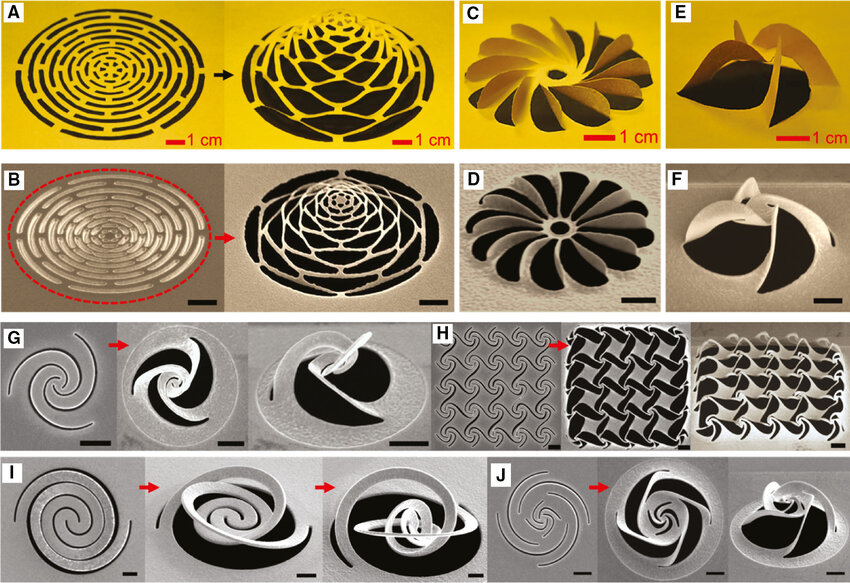
\includegraphics[height=0.55\textheight]{figures/kirigami_example.jpg}
		\caption{Example of macroscale Kirigami designs implemented on a microscale using a focused ion beam. Black scale bars: \SI{1}{\mu m}. Reproduced from~\cite{Li_2018}.}
	\end{figure}	
\end{frame}
%
%%% New frame %%%
%
\begin{frame}{Motivation}
	\framesubtitle{Out-of-plane buckling}
	\vspace{0.5cm}
	
	\begin{itemize}
		\item Out-of-plane buckling
		\item Surface properties are important for friction
		% \item Hanakata et al. \cite{Hanakata_2018,Hanakata_2020} found out-of-plane buckling with Kirigami designs
		% \item Surface properties are predicted to be important for friction properties
		\begin{itemize}
			\item Asperity theory: Contact area
			% \item Frenkel–Kontorova models: Commensurability
		\end{itemize}
	\end{itemize}
	% \vspace{1cm}

	\begin{figure}[H]
		\centering
		\begin{subfigure}[b]{0.49\textwidth}
			\centering
			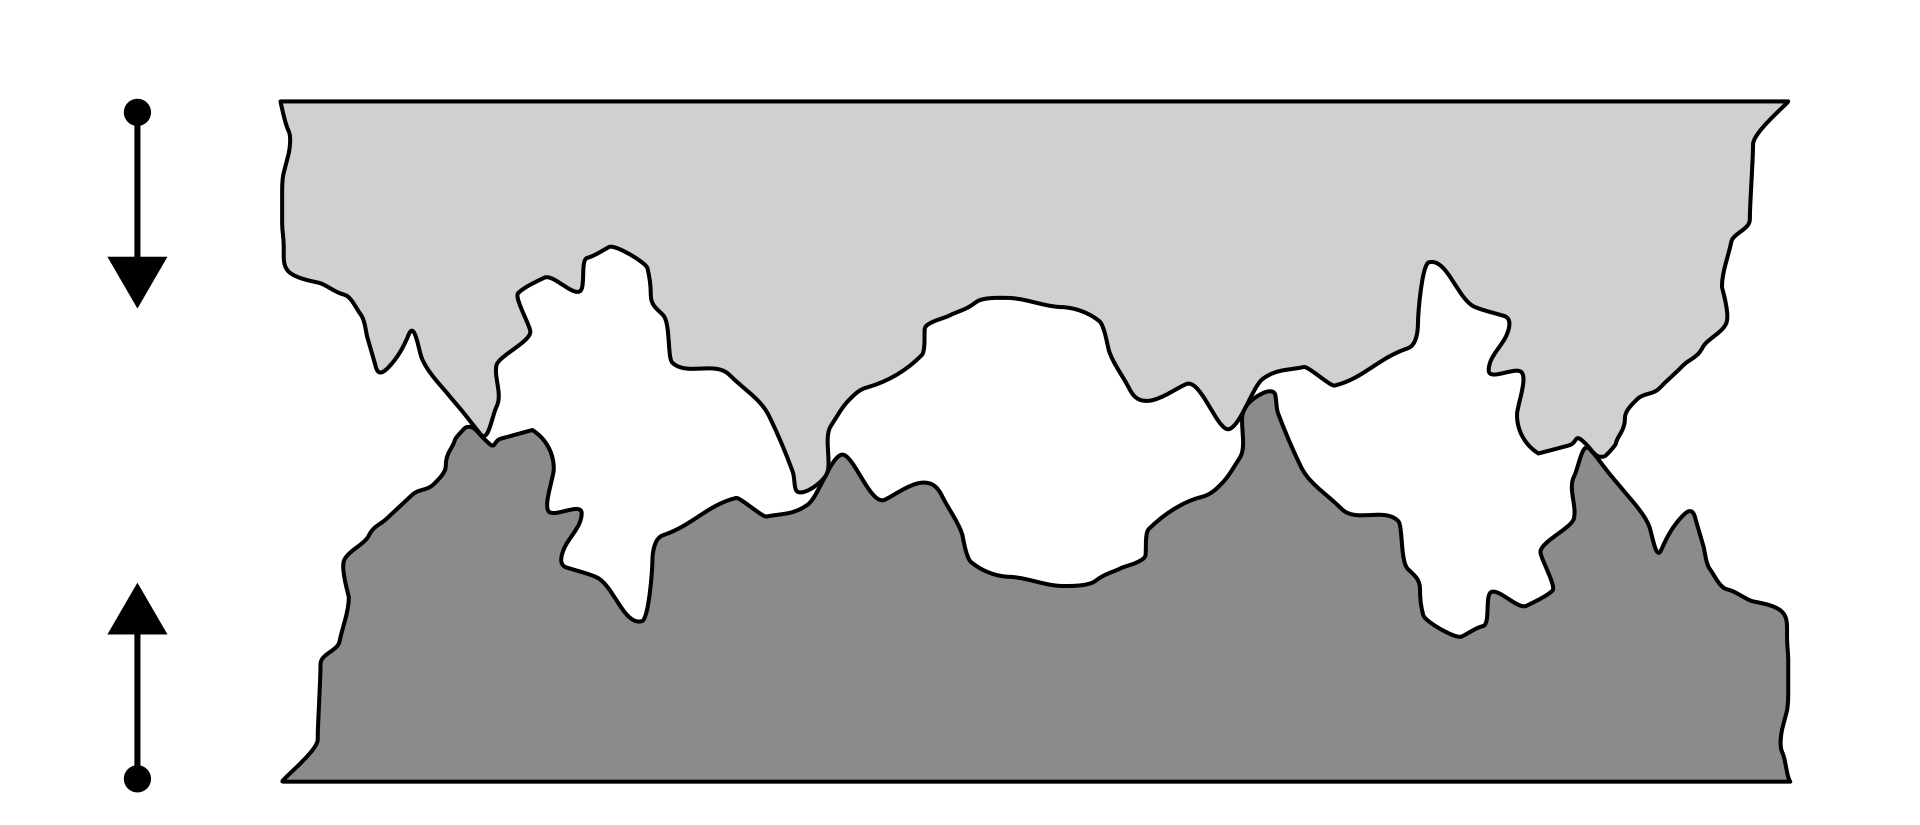
\includegraphics[width=\textwidth]{../thesis/figures/theory/asperities_top.png}
			\caption{Small load.}
			\label{fig:asp_left}
		\end{subfigure}
		\hfill
		\begin{subfigure}[b]{0.49\textwidth}
			\centering
			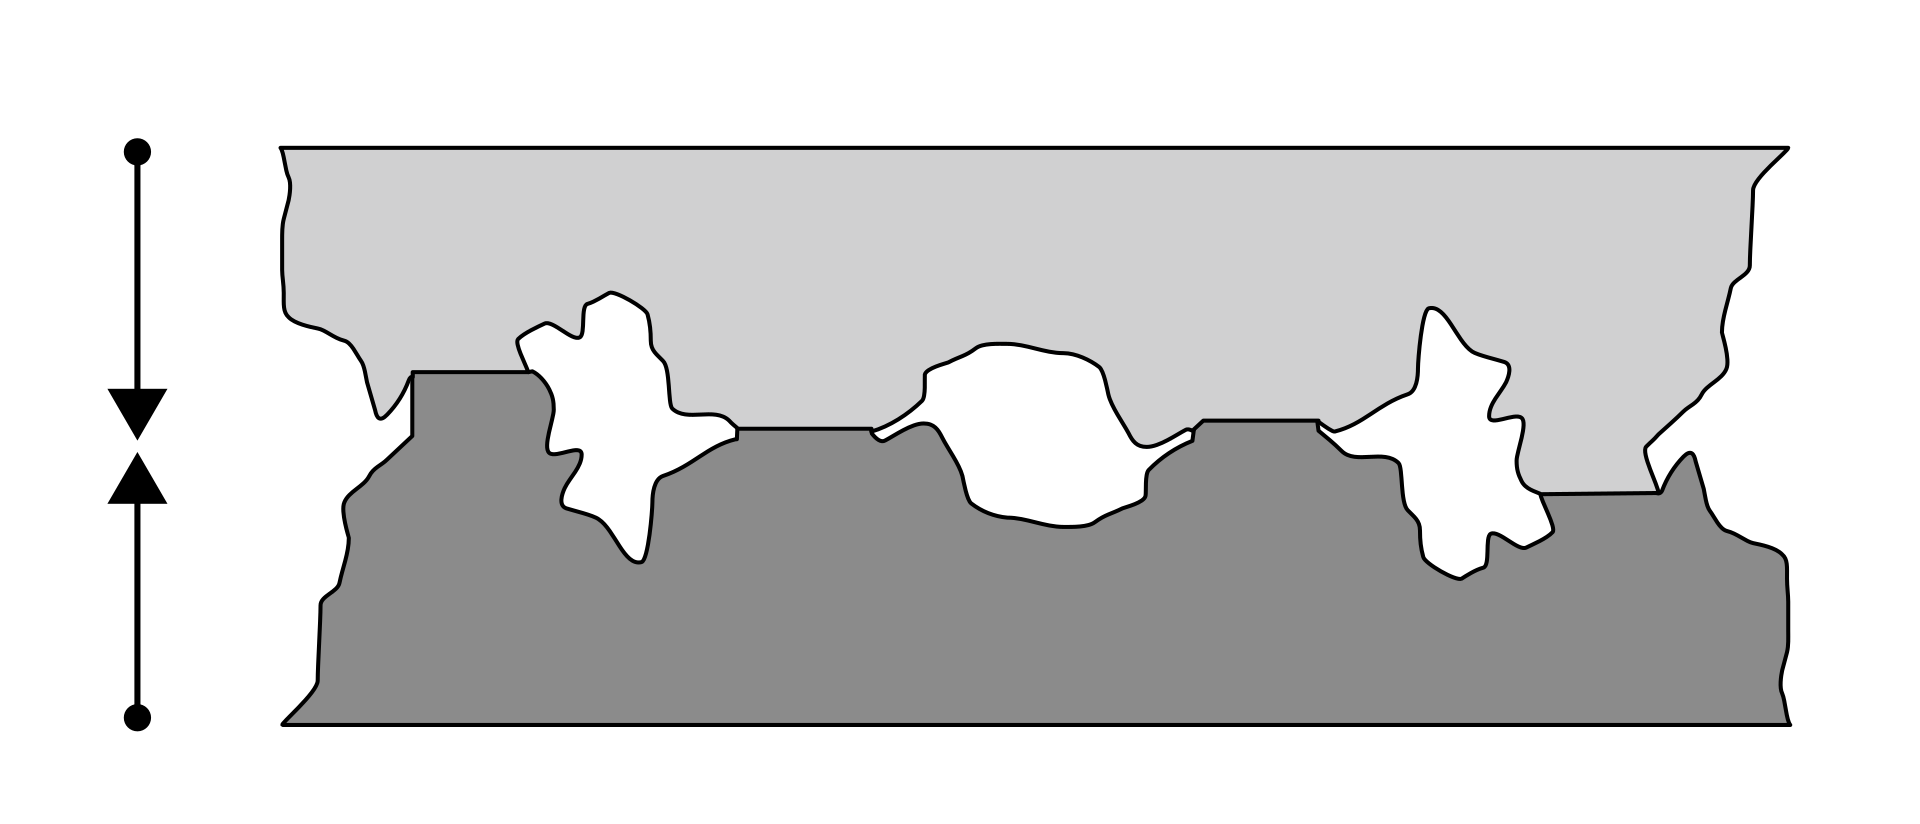
\includegraphics[width=\textwidth]{../thesis/figures/theory/asperities_bottom.png}
			\caption{High load.}
			\label{fig:asp_right}
		\end{subfigure}
		\caption{Qualitative illustration of microscopic asperity deformation under increasing load. Reproduced from~\cite{wiki:asperities}.}
	\end{figure}
\end{frame}
%
%%% New frame %%%
%
% \begin{frame}{Motivation}
% \framesubtitle{Contact area and commensurability}
% \begin{figure}[H]
% 	\centering
% 	\begin{subfigure}[b]{0.46\textwidth}
% 		\centering
% 		\includegraphics[width=\textwidth]{figures/nano_asperity_contact.png}
% 		\caption{Numerical MD results using an amorphous carbon tip and a diamond sample. Reproduced from~\cite{mo_friction_2009} with permission from Springer Nature.}
% 	\end{subfigure}
% 	\hfill
% 	\begin{subfigure}[b]{0.49\textwidth}
% 		\centering
% 		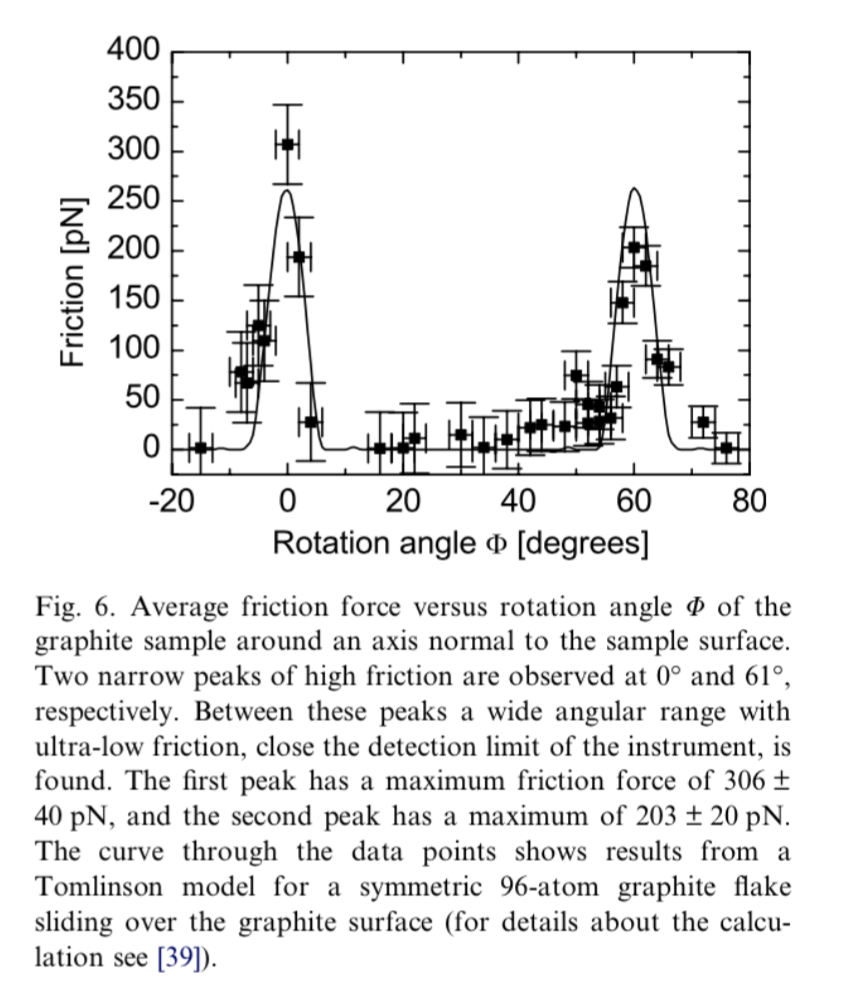
\includegraphics[width=\textwidth]{../thesis/figures/theory/graphene_rot.png}
% 		\caption{Experimental results of a graphene sheet sliding on graphite. Adapted from~\cite{DIENWIEBEL2005197}, reproduced from~\cite{Vanossi_2013} with permission from the American Physical Society.}
% 	\end{subfigure}
% 	% \caption{}
% \end{figure}
% \end{frame}
%
%%% New frame %%%
%


\section{Creating a graphene Kirigami system} %%%%%%%%%%%%%%%%%%%%%%%%%%%%%%%%%%%%%%%%%%%%%%%%%%%%%%%%%%%%%
\begin{frame}{Creating a graphene Kirigami system}
    \tableofcontents[currentsection]
\end{frame}


% \subsection{System setup}
% \begin{frame}{System setup}
% % \framesubtitle{System setup}
% 	\begin{figure}
% 		\centering    
% 		\movie[open,showcontrols=true,repeat]{\includegraphics[height=0.5\textwidth, keepaspectratio]{figures/sim_parts.png}}{figures/sim_parts.mov}
% 		\caption{System of choice: Graphene sheet on a silicon substrate. Blue: Substrate, Red: Inner sheet, Grey: Pull blocks. }
% 	\end{figure} 
% \end{frame}
%
%%% New frame %%%
%
\begin{frame}{System setup}
% \framesubtitle{System setup}
	\begin{columns} 
		\hspace{5mm}
		\begin{column}{.4\textwidth}
			Regions
			\begin{itemize}
				\item Red: $NVE$
				\item Green: Thermostat $NVT$
				\item Blue: Rigid 
			\end{itemize}
			\vspace*{5mm}
			System size
			\begin{itemize}
				\item Atoms $\sim 60,000$
				\item Sheet $\sim 130 \times \SI{165}{\text{Å}}$
			\end{itemize}
		\end{column}
		\begin{column}{.5\textwidth}
			\begin{figure}[H]
				\raggedright
				% \centering
				\begin{subfigure}[b]{0.9\textwidth}
					\centering
					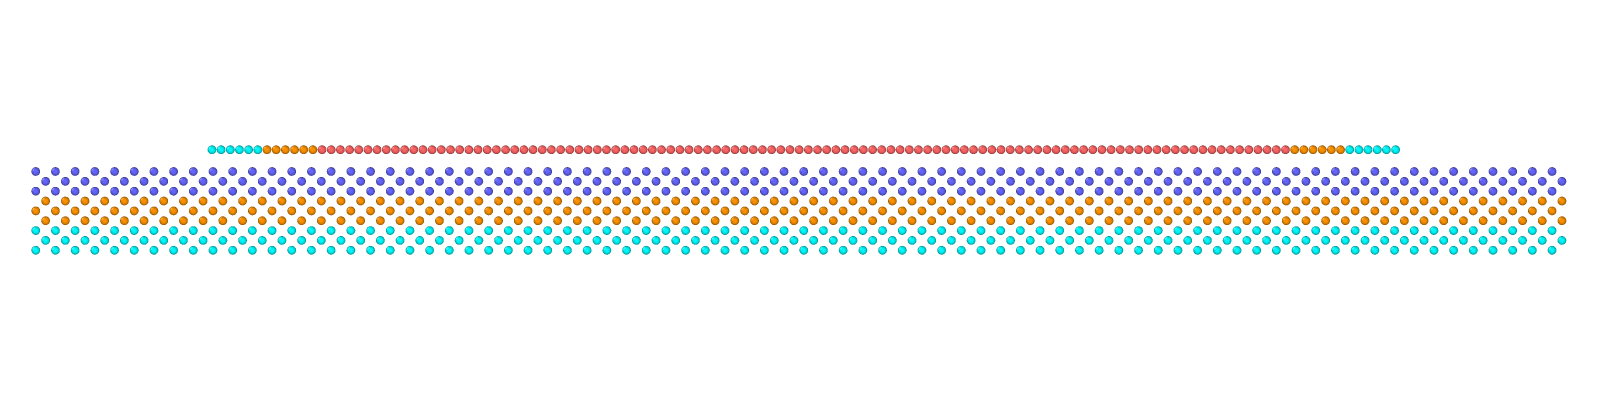
\includegraphics[width=\textwidth]{../thesis/figures/system/system_sideview.png}
					\caption{Side view.}
				\end{subfigure}
				\begin{subfigure}[b]{0.9\textwidth}
					\centering
					\includegraphics[width=\textwidth]{../thesis/figures/system/system_topview_anno.png}
					\caption{Top view.}
				\end{subfigure}
			\end{figure}
		\end{column}%
	\end{columns}	
\end{frame}
%
%%% New frame %%%
%

% \subsection{Kirigami design}
\begin{frame}{Sheet Kirigami}
	\framesubtitle{Indexing}
	\begin{align*}
		M \in \mathbb{Z}_2^{62 \times 106}, \qquad \text{Combinations} = 2^{6572} = 10^{1978}
	\end{align*}
	% \vspace*{5mm}
	\begin{figure}[H]
		\centering
		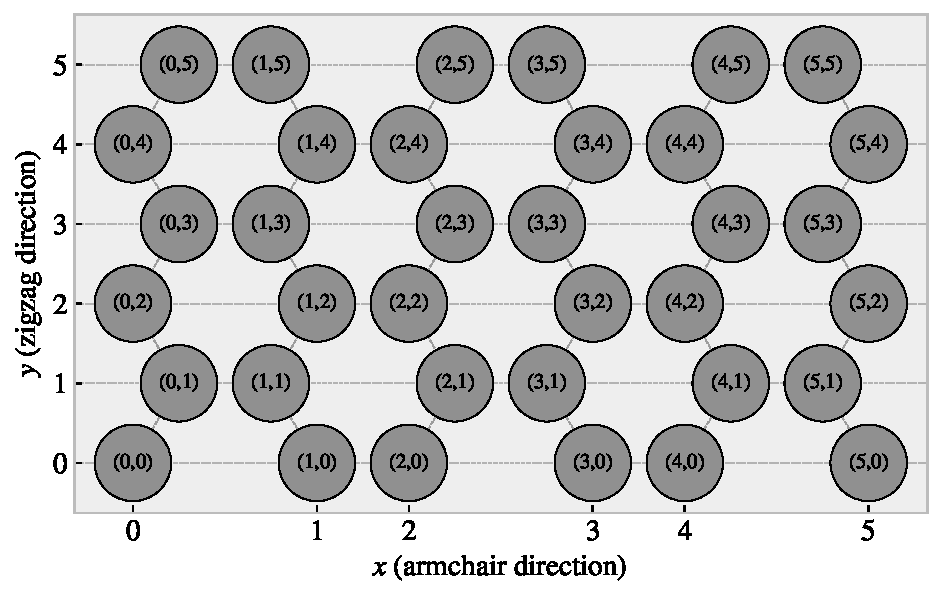
\includegraphics[width=0.7\linewidth]{../thesis/figures/system/atom_indexing.pdf}
		\caption{Graphene atom site indexing.}
	\end{figure}	
\end{frame}
%
%%% New frame %%%
%
% \begin{frame}{Sheet Kirigami}
% 	\framesubtitle{Indexing}
% 	% \vspace*{5mm}
% 	\begin{align*}
% 		M \in \mathbb{Z}_2^{62 \times 106}, \qquad \text{Combinations} = 2^{6572} = 10^{1978}
% 	\end{align*}
% 	\begin{figure}[H]
% 		\centering
% 		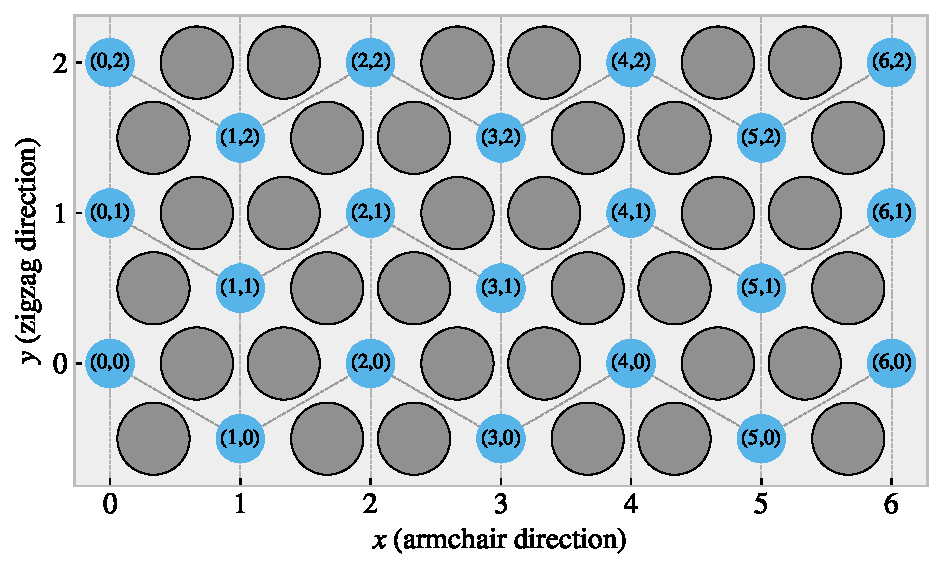
\includegraphics[width=0.7\linewidth]{../thesis/figures/system/center_indexing.pdf}
% 		\caption{Graphene \textit{center element} indexing.}
% 	\end{figure}	
% \end{frame}
%
%%% New frame %%%
%
\begin{frame}{Sheet Kirigami}
	\framesubtitle{Macroscale inspiration}
	\vspace*{5mm}
	\begin{figure}[H]
		\centering
		\begin{subfigure}[t]{0.48\textwidth}
			\centering
			\includegraphics[width=\textwidth]{../thesis/figures/system/pop_up_inspiration.png}
			\caption{Tetrahedron: Alternating perpendicular cuts producing a tetrahedron-shaped surface buckling when stretched. Reproduced from~\cite{new_pop_up}. }
		\end{subfigure}
		\hfill
		\begin{subfigure}[t]{0.48\textwidth}
			\centering
			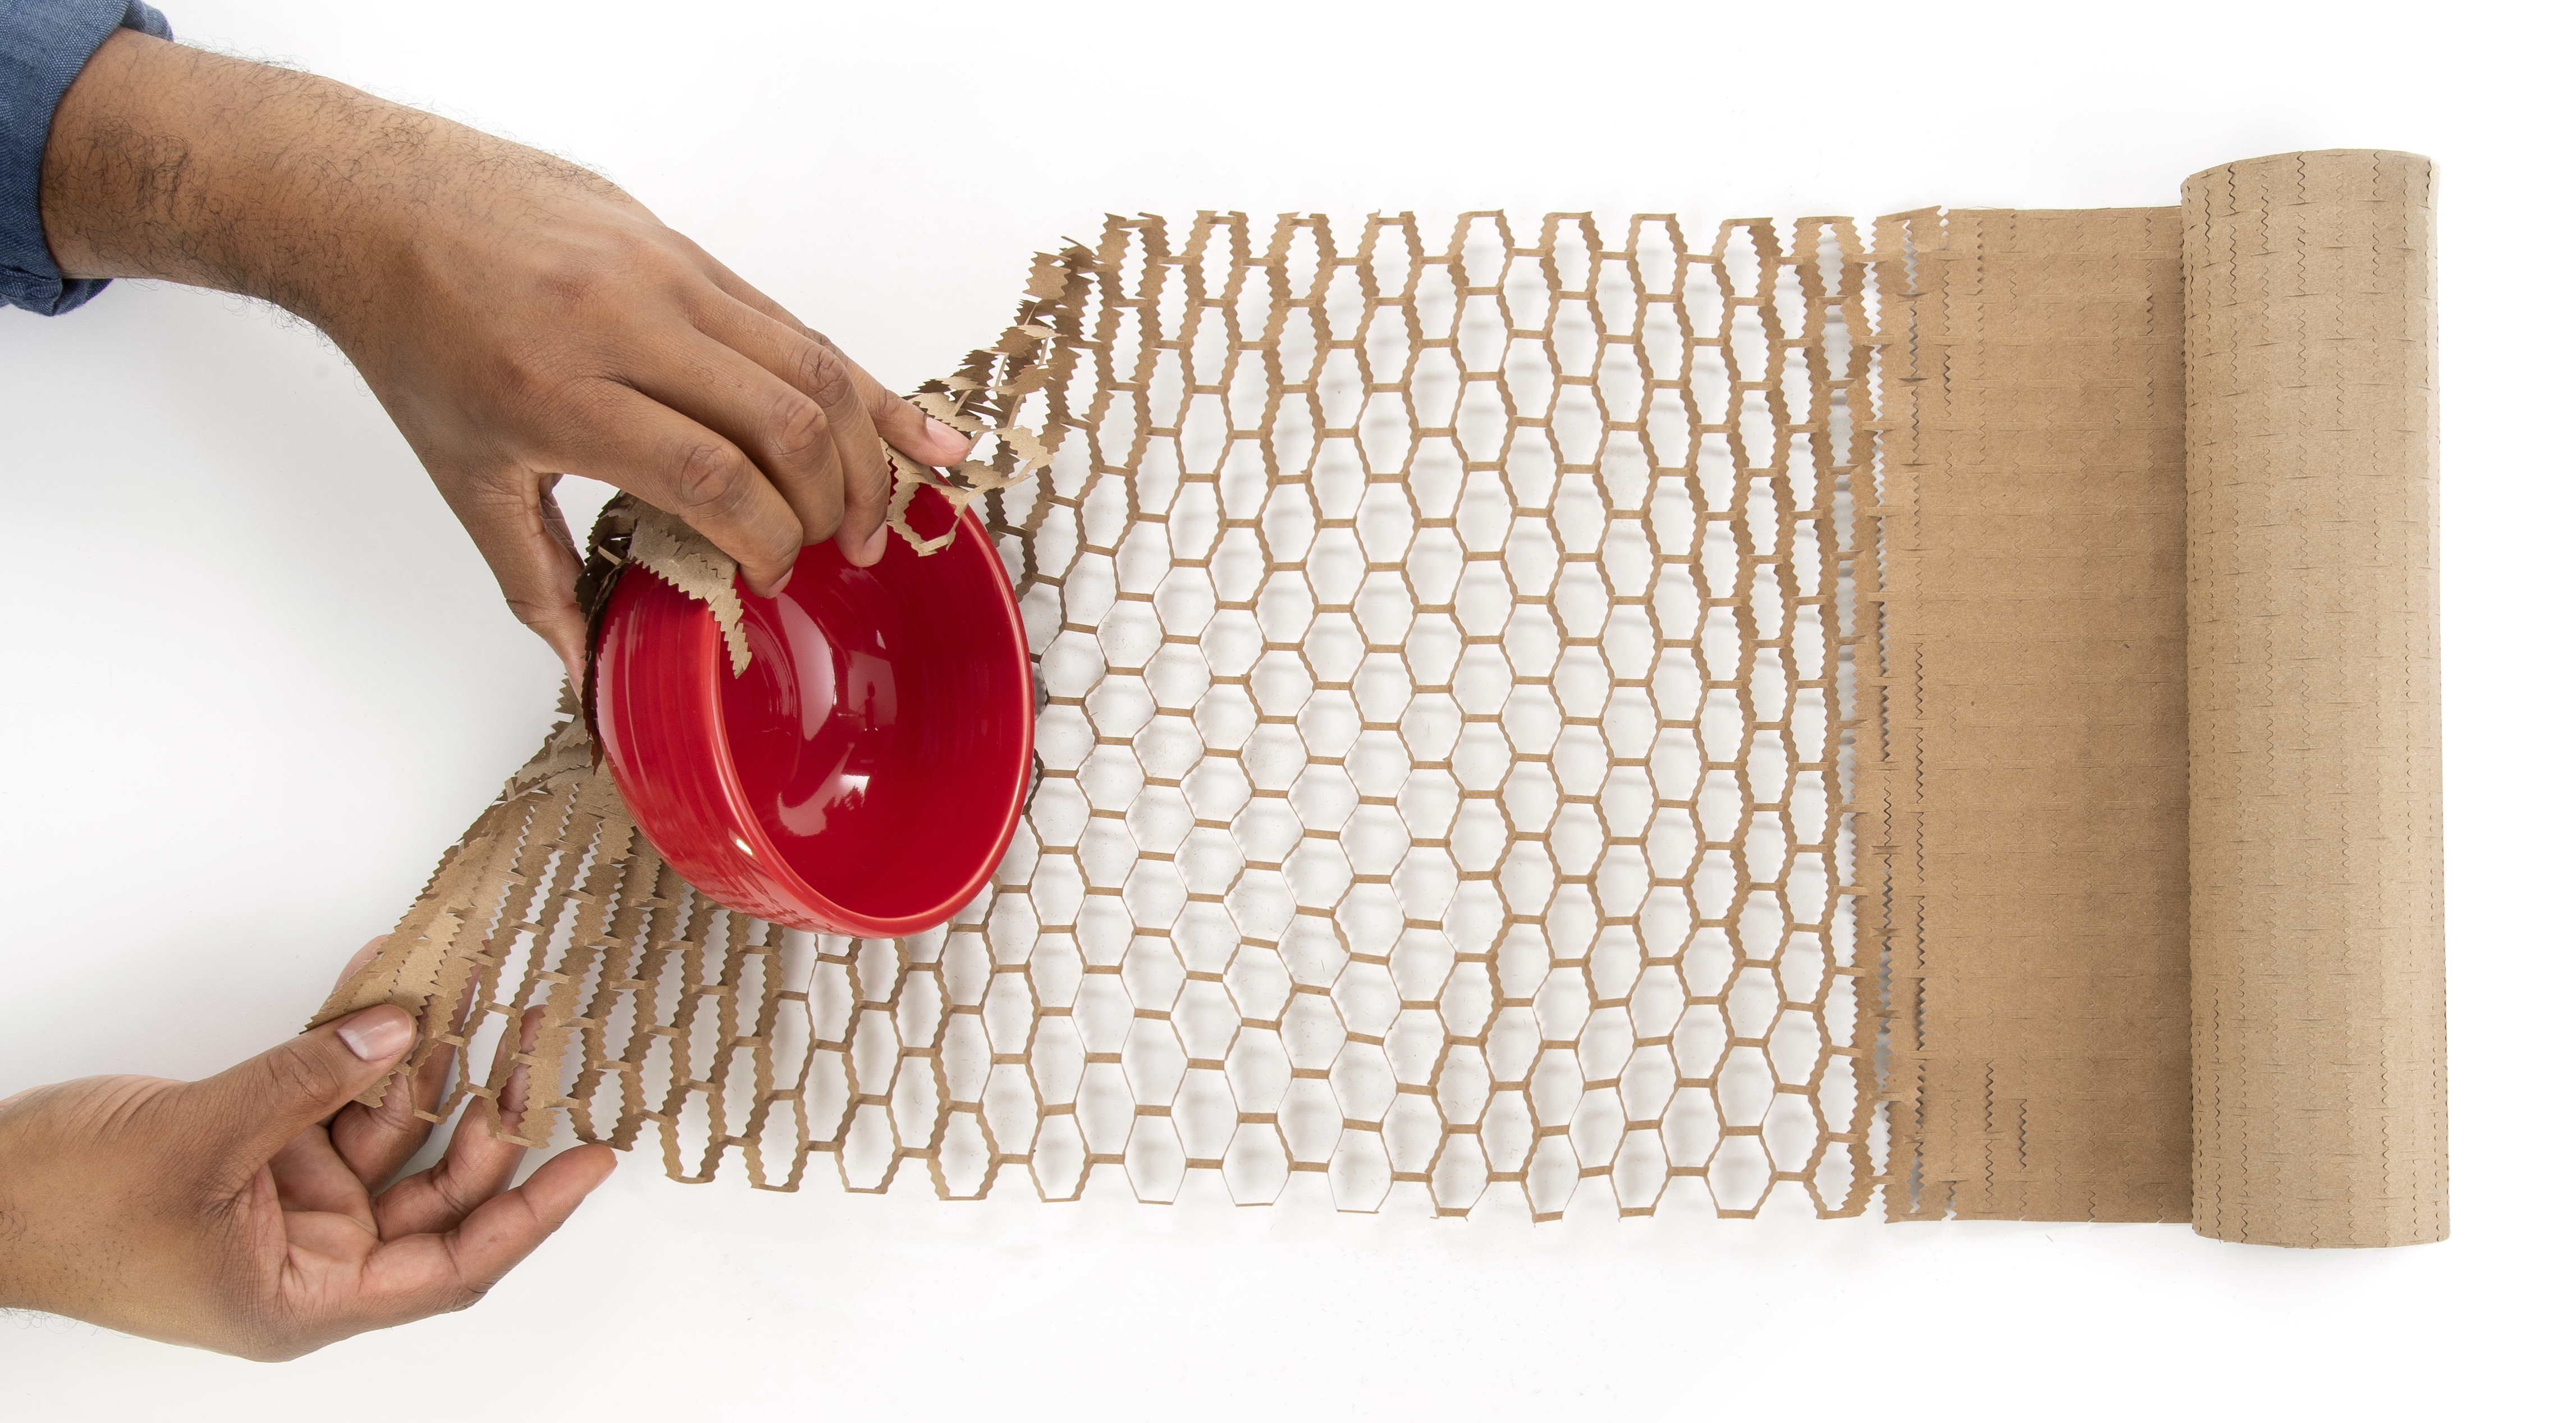
\includegraphics[width=\textwidth]{../thesis/figures/system/honeycomb_inspiration.jpg}
			\caption{Honeycomb: Scotch\textsuperscript{TM} Cushion Lock\textsuperscript{TM}~\cite{cushion_wrap} producing a honeycomb-shaped surface buckling when stretched. Reproduced from~\cite{cushion_wrap}.}
		\end{subfigure}
		\hfill
		\caption{Macroscale kirigami cut patterns used as inspiration for the nanoscale implementation.}
	  \end{figure}
\end{frame}
%
%%% New frame %%%
%
\begin{frame}{Sheet Kirigami}
	\framesubtitle{Tetrahedron patterns}

	\begin{figure}[H]
		\centering
		\begin{subfigure}[t]{0.49\textwidth}
			\centering
			\raggedleft
			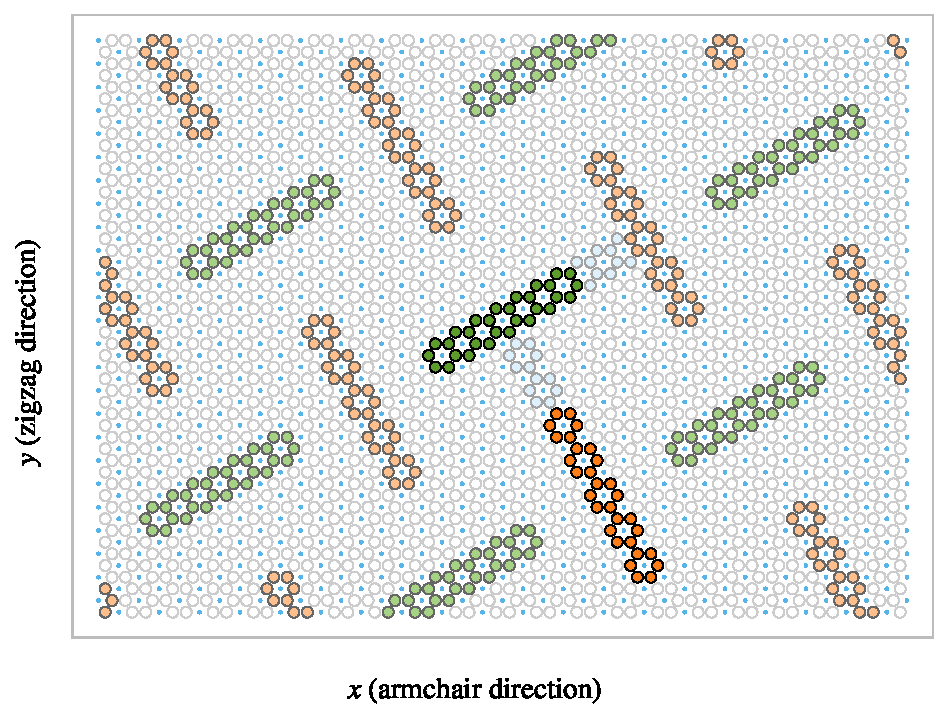
\includegraphics[width=0.7\textwidth]{../thesis/figures/system/pop_up_inverse.pdf}
			% \caption{}
		  \end{subfigure}
		  \hfill
		  \begin{subfigure}[t]{0.49\textwidth}
			\centering
			\raggedright
			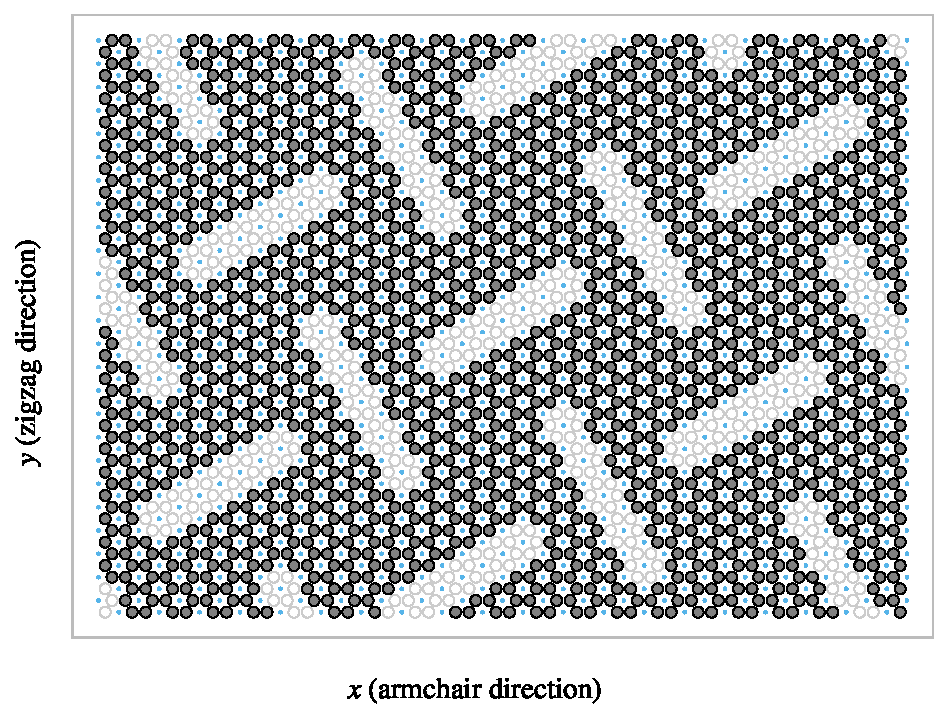
\includegraphics[width=0.7\textwidth]{../thesis/figures/system/pop_up_pattern.pdf}
			% \caption{}
		\end{subfigure}
	  \end{figure}
	  
	  
	  \begin{figure}[H]
		\centering
		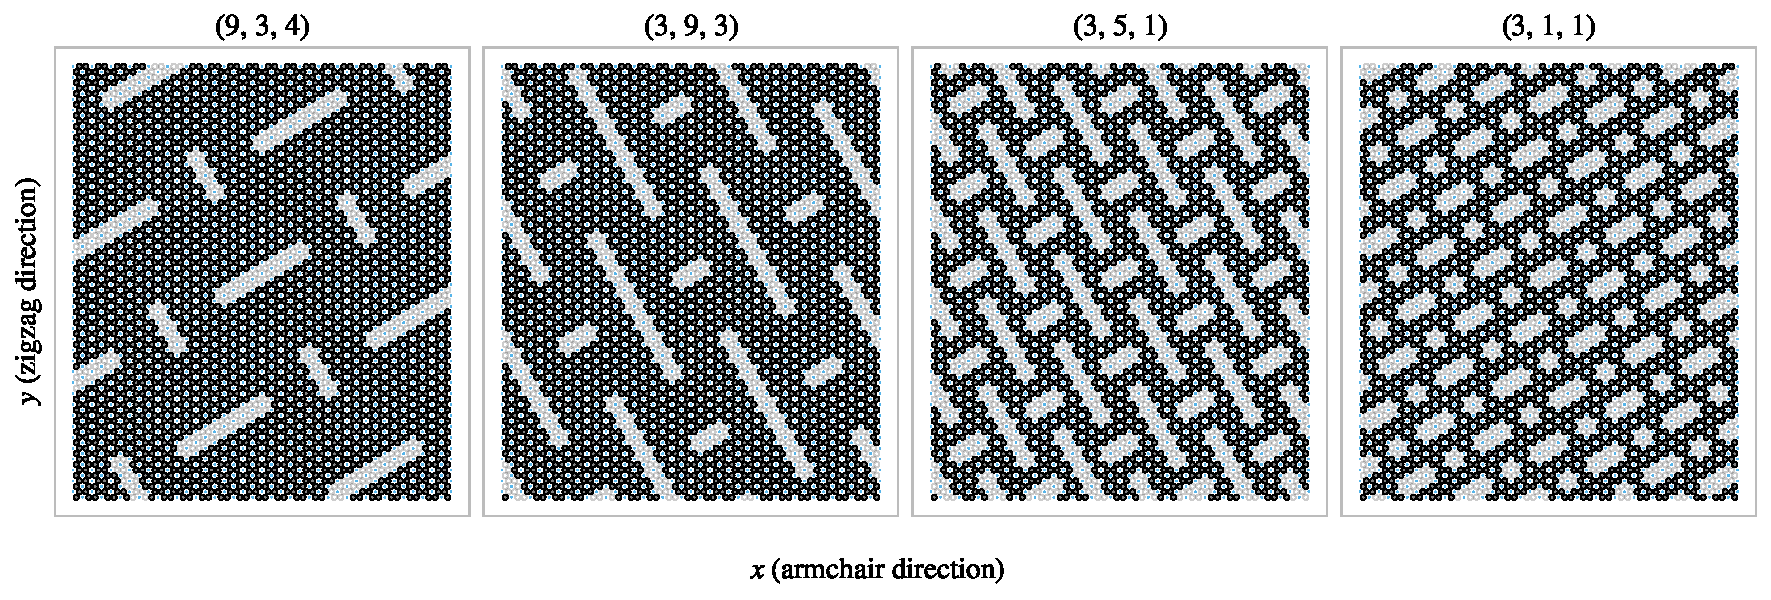
\includegraphics[trim={0 0 0 8mm},clip,width=\linewidth]{../thesis/figures/system/pop_up_flavors.pdf}
	  \end{figure}
	  
\end{frame}
%
%%% New frame %%%
%
\begin{frame}{Sheet Kirigami}
	\framesubtitle{Honeycomb patterns}

	\begin{figure}[H]
		\centering
		\begin{subfigure}[t]{0.48\textwidth}
			\centering
			\raggedleft
			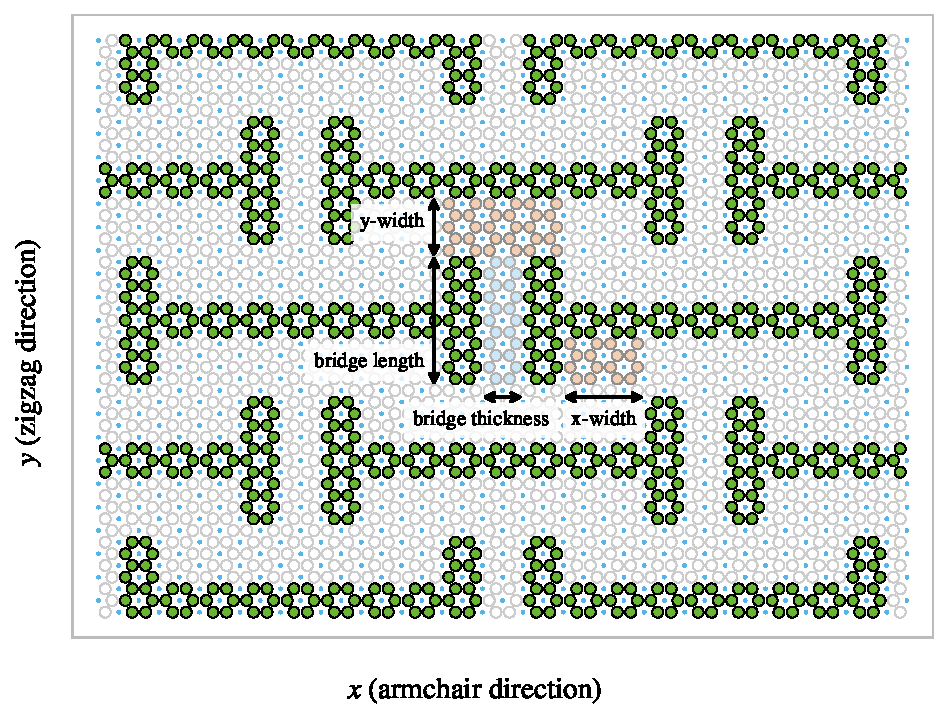
\includegraphics[width=0.7\textwidth]{../thesis/figures/system/honeycomb_inverse.pdf}
		  \end{subfigure}
		  \hfill
		  \begin{subfigure}[t]{0.48\textwidth}
			\centering
			\raggedright
			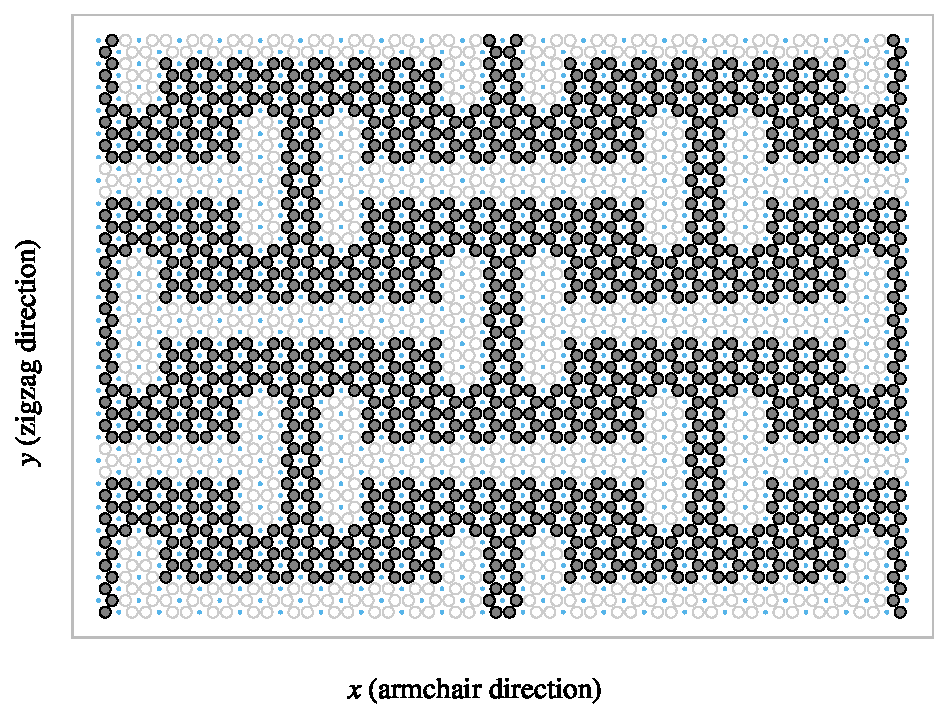
\includegraphics[width=0.7\textwidth]{../thesis/figures/system/honeycomb_pattern.pdf}
		\end{subfigure}
	  \end{figure}
	  
	  
	  \begin{figure}[H]
		\centering
		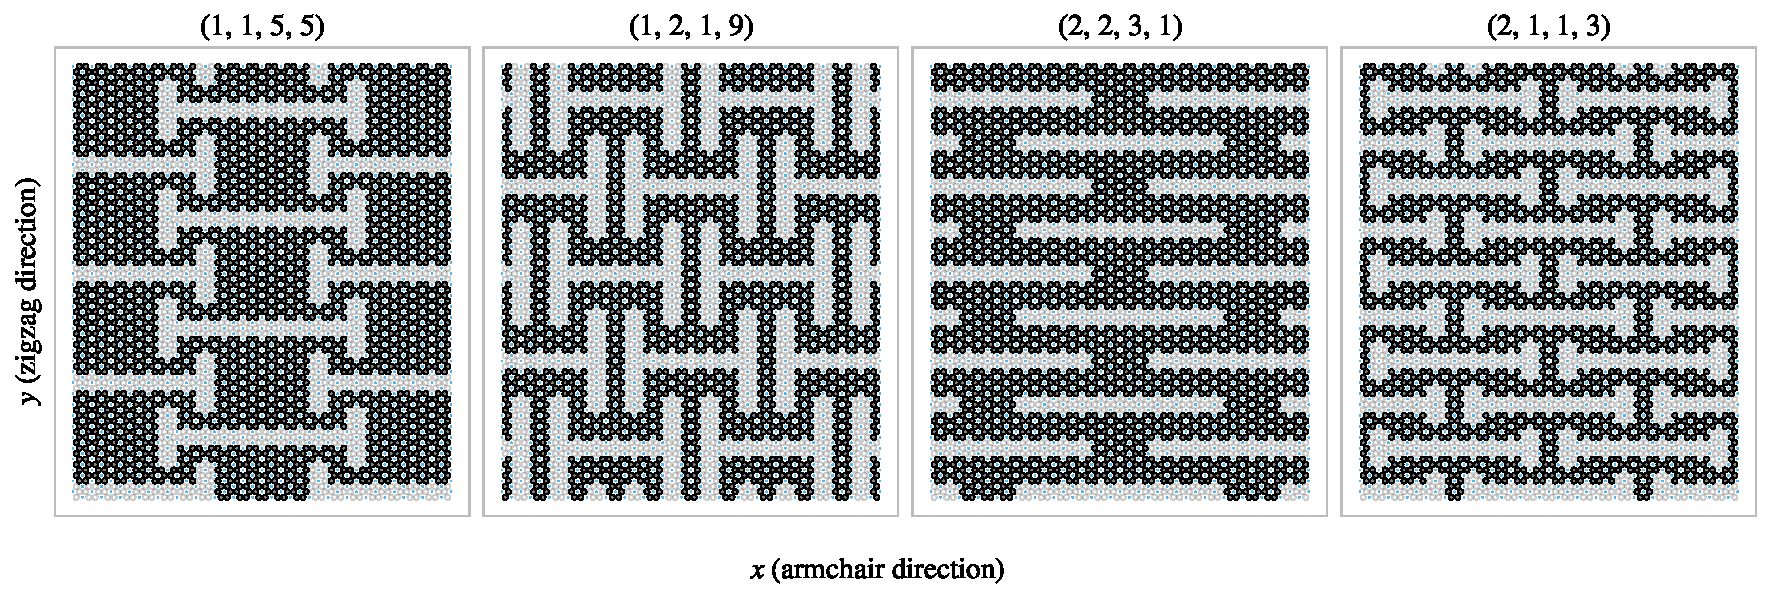
\includegraphics[trim={0 0 0 8mm},clip,width=\linewidth]{../thesis/figures/system/honeycomb_flavors.pdf}
	  \end{figure}
\end{frame}
%
%%% New frame %%%
%
\begin{frame}{Sheet Kirigami}
	\framesubtitle{Random walk patterns}
	\begin{figure}[H]
		\centering
		\includegraphics[width=0.8\linewidth]{../thesis/figures/system/RW_flavors.png}
	\end{figure}
\end{frame}
%
%%% New frame %%%
%

% \begin{frame}{Molecular Dynamics (MD)}
% 	\begin{itemize}
% 		\item Newtons equations (NVE)
% 		\begin{align*}
% 			m_i \frac{d^2 \vec{r}_i}{dt^2} = \vec{F}_i = -\nabla U_i,
% 		\end{align*}
% 		\item Introducing temperature (NVT) with the Langevin equation
% 		\begin{align*}
% 			m_i \frac{d^2 \vec{r}_i}{dt^2} &= \underbrace{\strut -\nabla U_i}_{F_i} \quad \underbrace{\strut -\alpha \vec{v}_i}_{\text{Drag}} \quad  + \underbrace{\strut \vec{R}_i}_{\text{Fluctuation}}, \\
% 			\\
% 			\langle R \rangle &= 0, \qquad \langle R^2 \rangle = 2\alpha k_B T.
% 		\end{align*}
% 	\end{itemize}
% \end{frame}


\section{Friction behaviour} %%%%%%%%%%%%%%%%%%%%%%%%%%%%%%%%%%%%%%%%%%%%%%%%%%%%%%%%%%%%%
\begin{frame}{Friction behaviour}
    \tableofcontents[currentsection]
\end{frame}

% \subsection{Friction metrics}
\begin{frame}{Friction metrics}
	\begin{figure}[H]
	\centering
	\begin{subfigure}[t]{0.49\textwidth}
		\centering
		\includegraphics[width=1\textwidth]{../thesis/figures/baseline/drag_Ff_10Å.pdf}
		\caption{\SI{10}{\text{Å}} sliding.}
	\end{subfigure}
	\hfill
	\begin{subfigure}[t]{0.49\textwidth}
		\centering
		\includegraphics[width=1\textwidth]{../thesis/figures/baseline/drag_Ff_100Å.pdf}
		\caption{\SI{100}{\text{Å}} sliding.}
	  \end{subfigure}
	   \caption{Friction force traces. The red line represents a Savgol filter.}
	%    \caption{Friction force traces. The red line represents a Savgol filter. \\ $T = \SI{300}{K}$, $v = \SI{20}{m/s}$, $K = \infty$.}
  \end{figure}
\end{frame}
% \begin{frame}{Friction metrics}
% 	\begin{figure}[H]
% 	\centering
% 	\begin{subfigure}[t]{0.49\textwidth}
% 		\centering
% 		\begin{columns}
% 			\column{.3\linewidth}
% 			% \hspace{5mm}
% 			\caption{\scriptsize \\ \vspace*{1mm}  $K = \infty$, \\ $v = \SI{20}{m/s}$ \\ (\SI{10}{\text{Å}} sliding).}
% 			\column{.7\linewidth}
% 			\includegraphics[width=1\textwidth]{../thesis/figures/baseline/drag_Ff_10Å.pdf}
% 		\end{columns}
% 	\end{subfigure}
% 	\hfill
% 	\begin{subfigure}[t]{0.49\textwidth}
% 		\centering
% 		\begin{columns}
% 			\column{.7\linewidth}
% 			\includegraphics[width=1\textwidth]{../thesis/figures/baseline/drag_Ff_100Å.pdf}
% 			\column{.3\linewidth}
% 			\caption{\scriptsize \\ \vspace*{1mm} $K = \infty$, \\ $v = \SI{20}{m/s}$ \\ (\SI{100}{\text{Å}} sliding).}
% 		\end{columns}
% 	  \end{subfigure}
% 	\hfill
% 	\begin{subfigure}[t]{0.49\textwidth}
% 		\centering
% 		\begin{columns}
% 			\column{.3\linewidth}
% 			\caption{\scriptsize \\ \vspace*{1mm} $K = \SI{10}{N/m}$, \\ $v = \SI{1}{m/s}$ \\ (\SI{10}{\text{Å}} sliding).}
% 			\column{.7\linewidth}
% 			\includegraphics[width=1\textwidth]{../thesis/figures/baseline/drag_Ff_10Å_K10_v1.pdf}
% 		\end{columns}
% 	\end{subfigure}
% 	\hfill
% 	\begin{subfigure}[t]{0.49\textwidth}
% 		\centering
% 		\begin{columns}
% 			\column{.7\linewidth}
% 			\includegraphics[width=1\textwidth]{../thesis/figures/baseline/drag_Ff_100Å_K10_v1.pdf}
% 			\column{.3\linewidth}
% 			\caption{\scriptsize \\ \vspace*{1mm}  $K = \SI{10}{N/m}$, \\ $v = \SI{1}{m/s}$ \\ (\SI{100}{\text{Å}} sliding).}
% 		\end{columns}
% 	\end{subfigure}
% 	   \caption{Friction force traces. The red line represents a Savgol filter.}
%   \end{figure}
% \end{frame}
%
%%% New frame %%%
%
% \subsection{Out-of-plane buckling}
\begin{frame}{Out-of-plane buckling}
	\begin{figure}
		\centering    
		\movie[open,showcontrols=true]{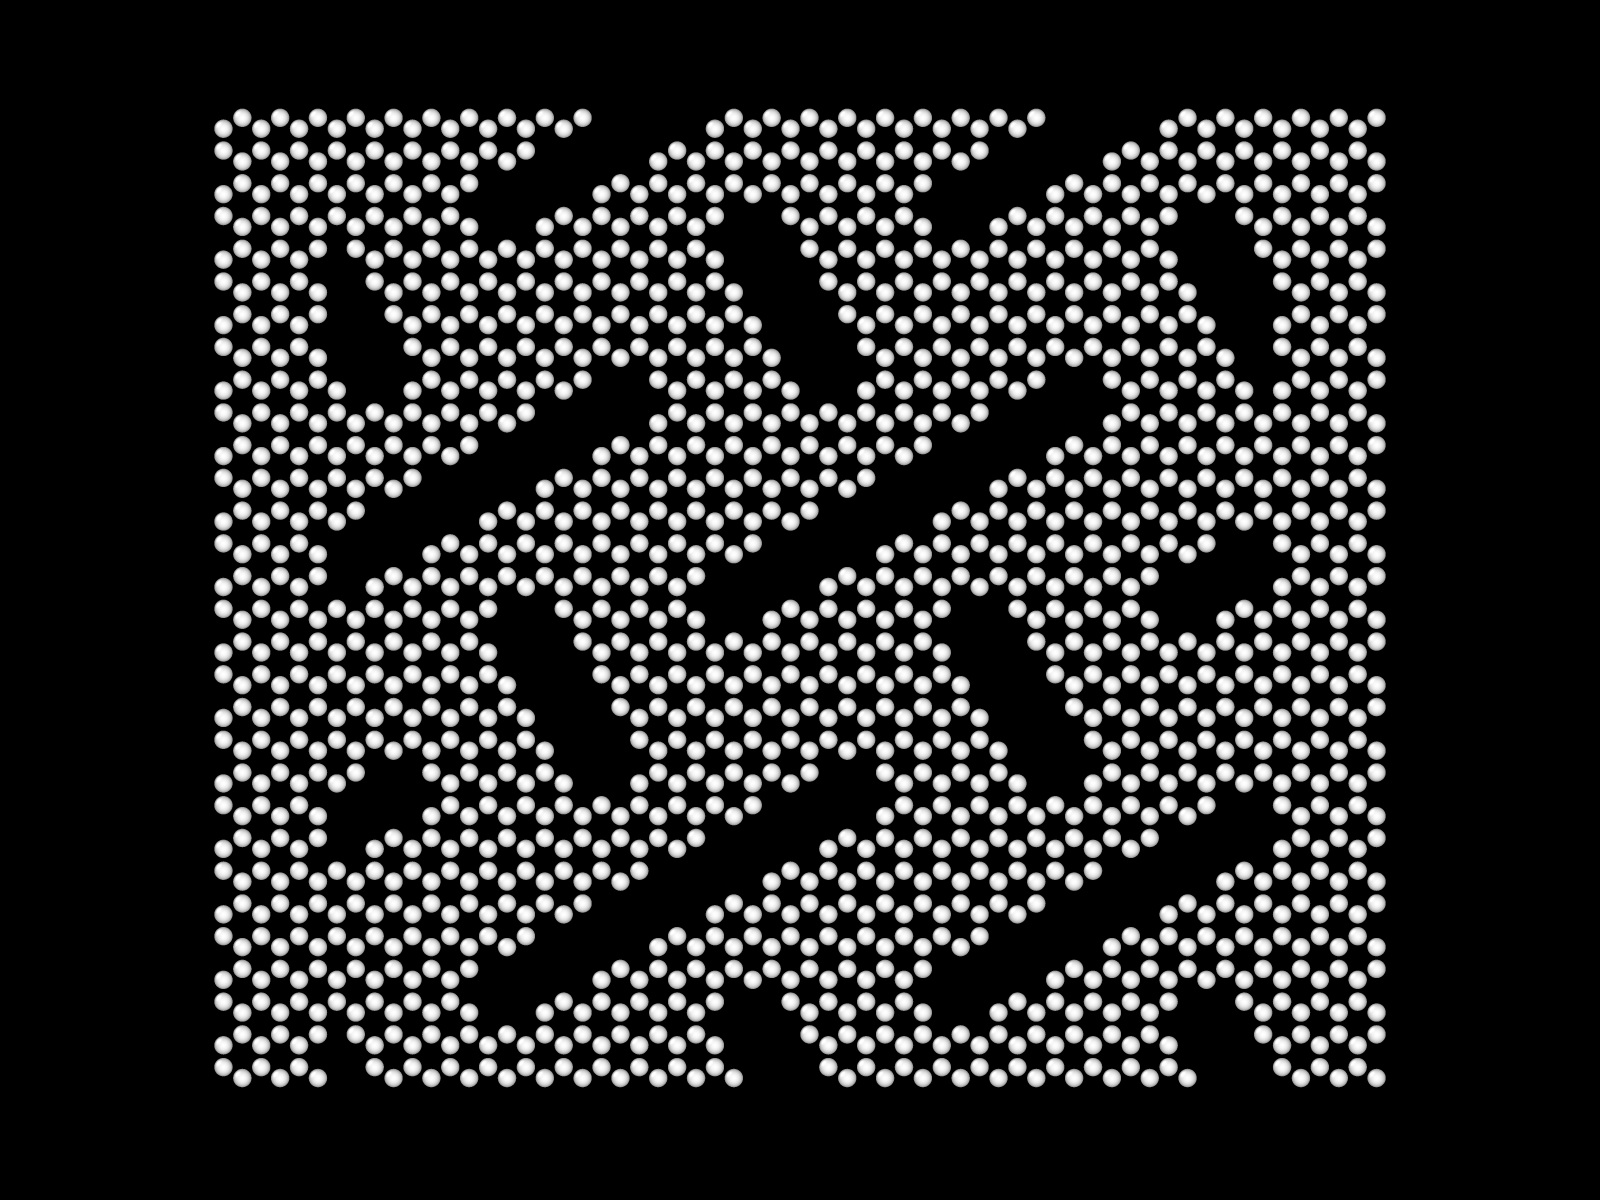
\includegraphics[height=0.7\textheight, keepaspectratio]{figures/vacuum_stretch.png}}{figures/vacuum_stretch.mov}
		\caption{Kirigami sheet stretch in a vacuum.}
	\end{figure} 

\end{frame}
%
%%% New frame %%%
%
\begin{frame}{Out-of-plane buckling}
	\begin{figure}
		\centering    
		\movie[open,showcontrols=true]{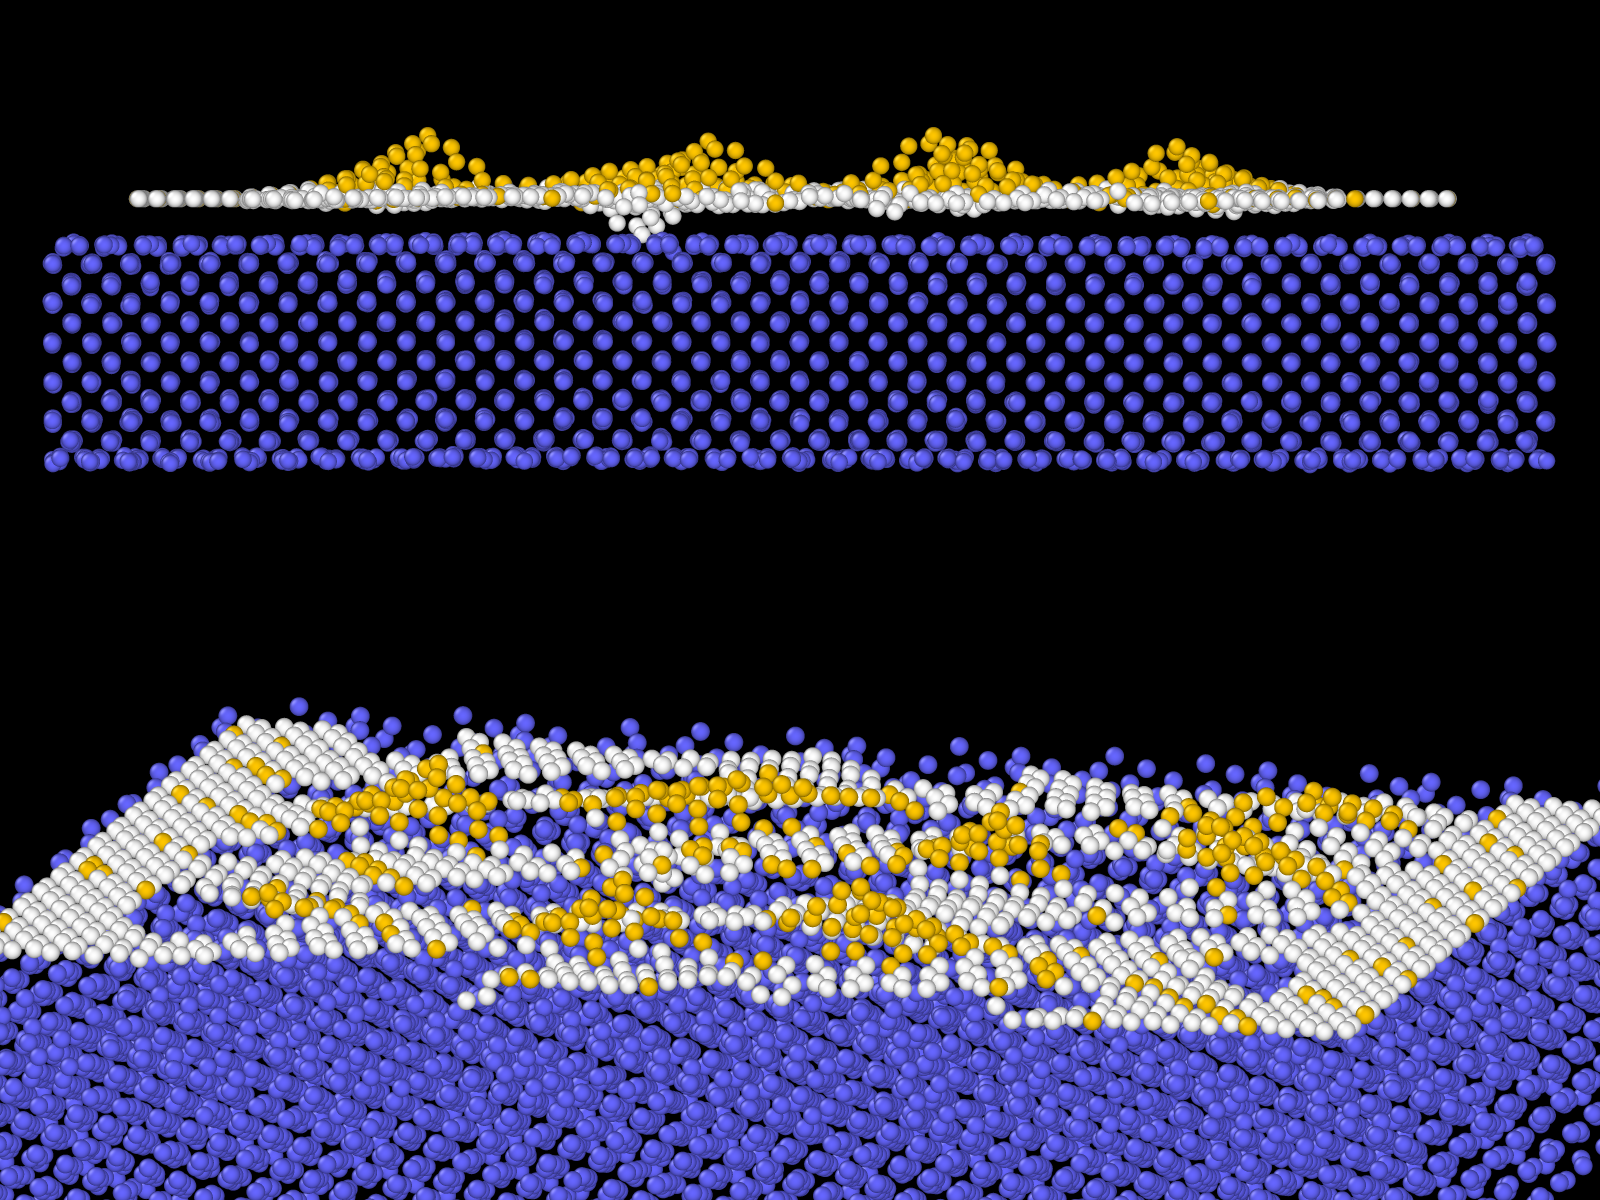
\includegraphics[height=0.7\textheight, keepaspectratio]{figures/contact_stretch.png}}{figures/contact_stretch.mov}
		\caption{Kirigami stretch in contact with the substrate.}
	\end{figure} 
\end{frame}
%
%%% New frame %%%
%
\begin{frame}{Out-of-plane buckling}
	\begin{figure}
		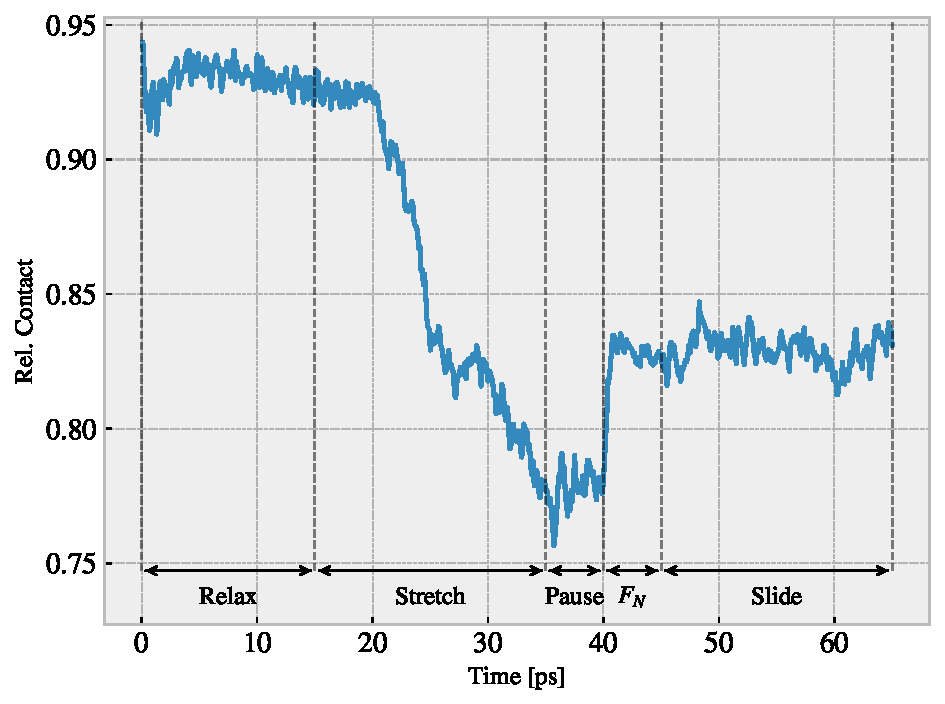
\includegraphics[height=0.7\textheight]{figures/contact_pct.pdf}
		\caption{Contact area approximation: Number of C--Si bonds within a threshold distance of 110\% the LJ interaction equilibrium distance.}
	\end{figure}	
\end{frame}


% \subsection{Strain profiles}
\begin{frame}{Contact-strain profile}

	\begin{figure}[H]
		\centering
		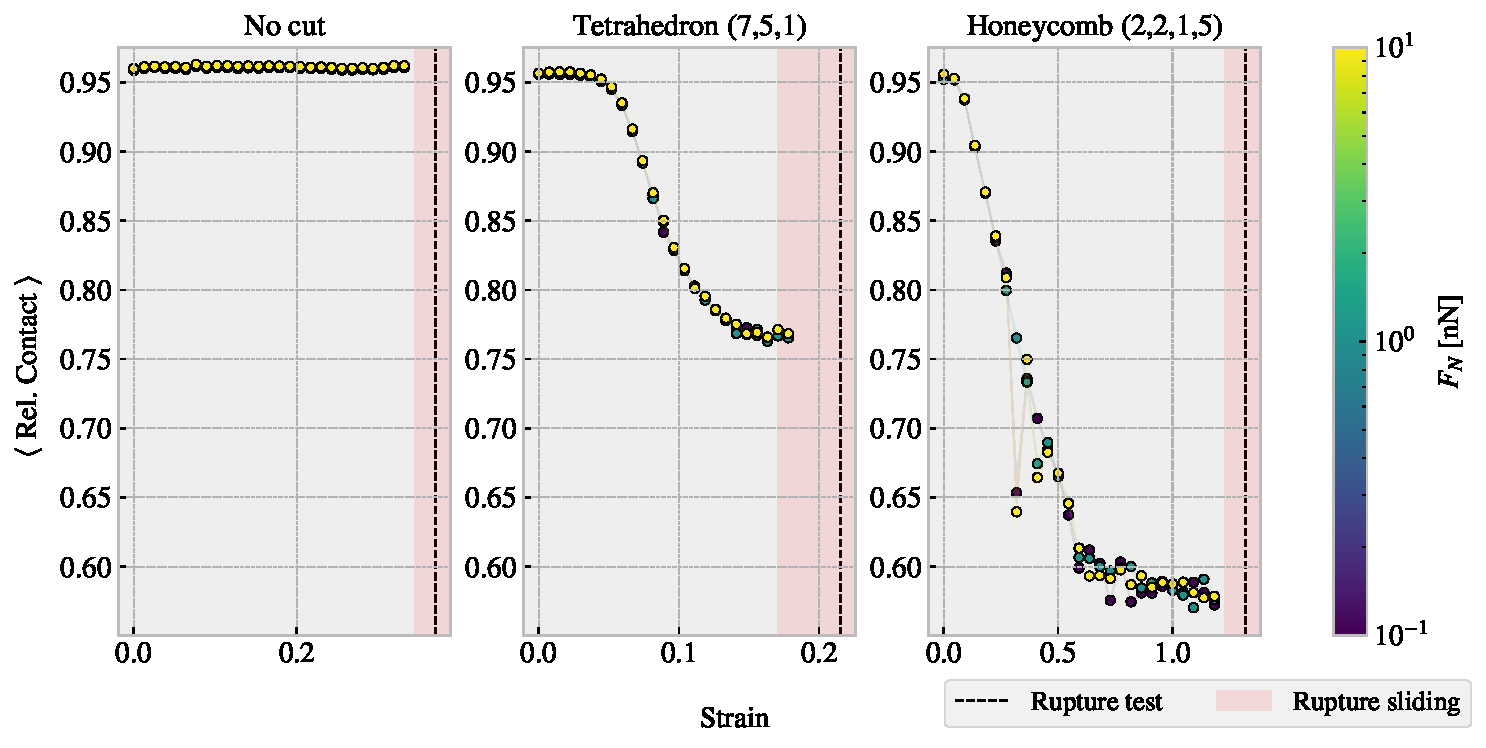
\includegraphics[width=1\linewidth]{../thesis/figures/baseline/multi_stretch_area_compare.pdf}
		\caption{Contact-strain profile for $F_N = \{0.1, 1, 10\} \text{nN}$.}
	\end{figure}
\end{frame}
%
%%% New frame %%%
%
\begin{frame}{Friction-strain profile}
	\begin{figure}[H]
		\centering
		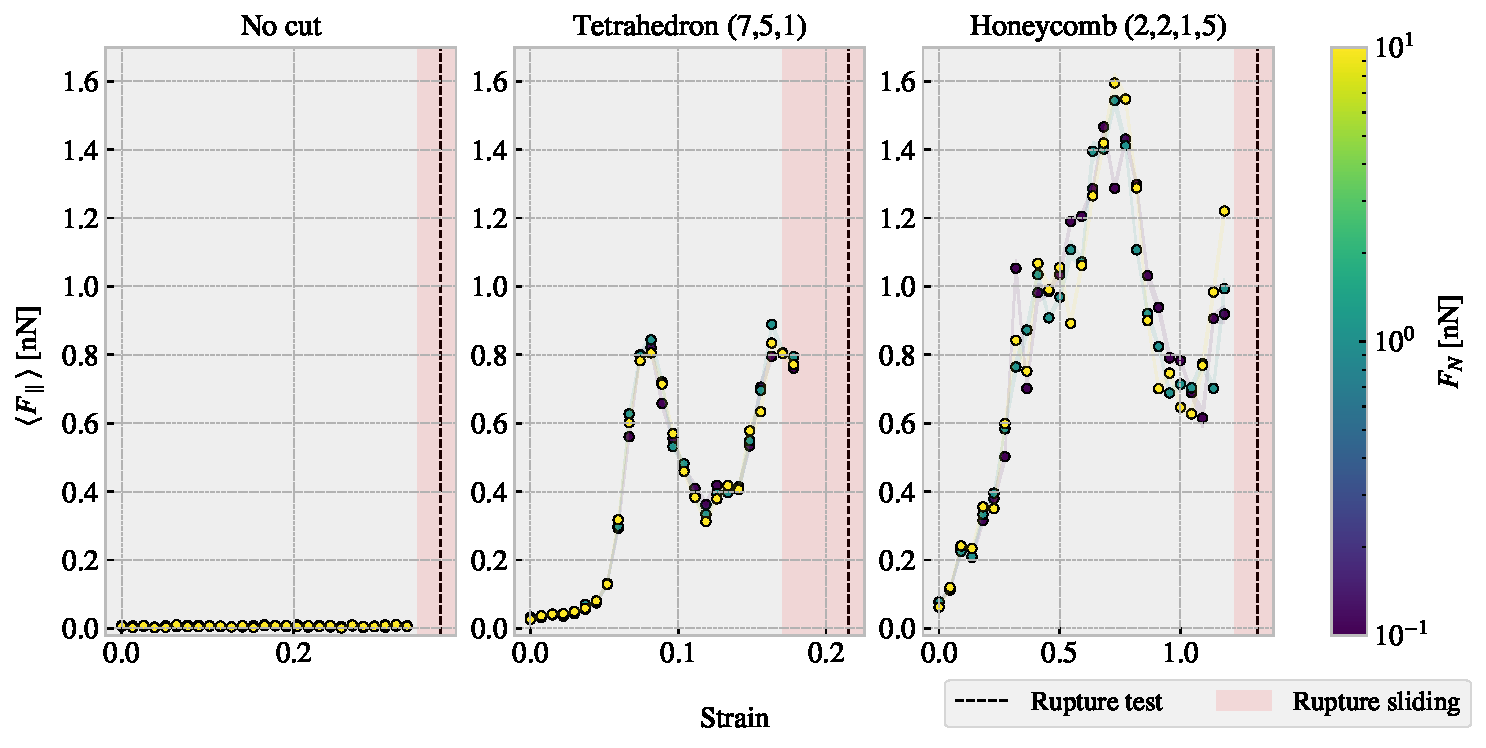
\includegraphics[width=1\linewidth]{../thesis/figures/baseline/multi_stretch_mean_compare.pdf}
		\caption{Friction-strain profile for $F_N = \{0.1, 1, 10\} \text{nN}$.}
	\end{figure}
\end{frame}
%
%%% New frame %%%
%
% \subsection{Negative friction coefficient}
\begin{frame}{Negative friction coefficient}
	Coupling of load to sheet tension 
	\begin{align*}
		F_t = T\cdot F_N, \qquad T = 6
	\end{align*}
	\begin{figure}[H]
		\centering
		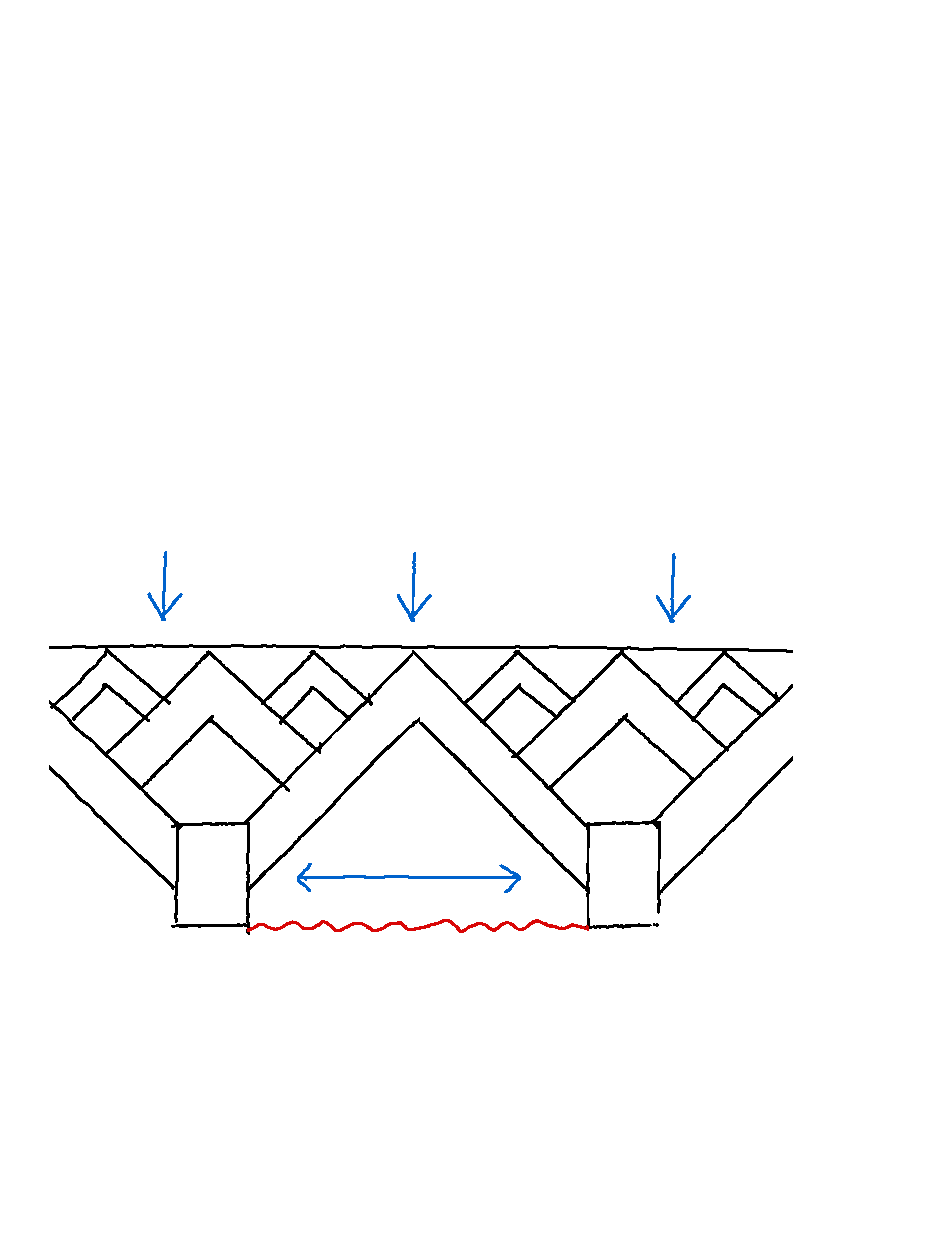
\includegraphics[width=0.6\linewidth]{../thesis/figures/negative_coefficient/nanomachine.pdf}
		\caption{Working sketch for a nanomachine design translating applied load to a strain of the sheet (shown in red).}
		% \caption{Working sketch for a nanomachine design translating applied load (from the top of the figure) to a straining of the graphene sheet (shown in red).}
		\label{fig:nanomachine}
	\end{figure}	  
\end{frame}
%
%%% New frame %%%
%
\begin{frame}{Negative friction coefficient}
	\framesubtitle{Tetrahedron results}
	
	\begin{figure}[H]
		\centering
		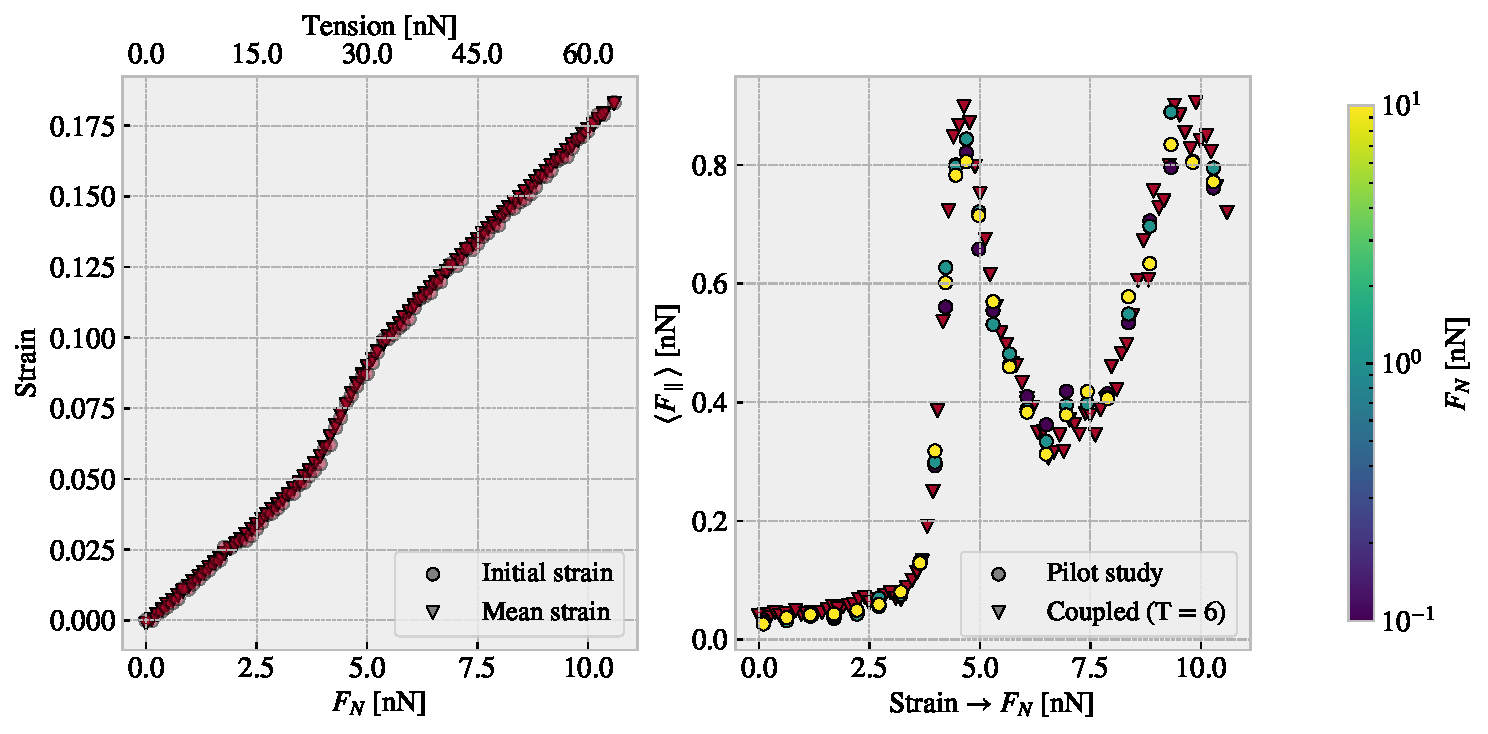
\includegraphics[width=\linewidth]{../thesis/figures/negative_coefficient/manual_coupling_tension_pop7_5_1.pdf}	
		\caption{Tetrahedron $(7,5,1)$}
	\end{figure}	
\end{frame}
%
%%% New frame %%%
%

\begin{frame}{Negative friction coefficient}
	\framesubtitle{Honeycomb results}
	\begin{figure}[H]
		\centering
		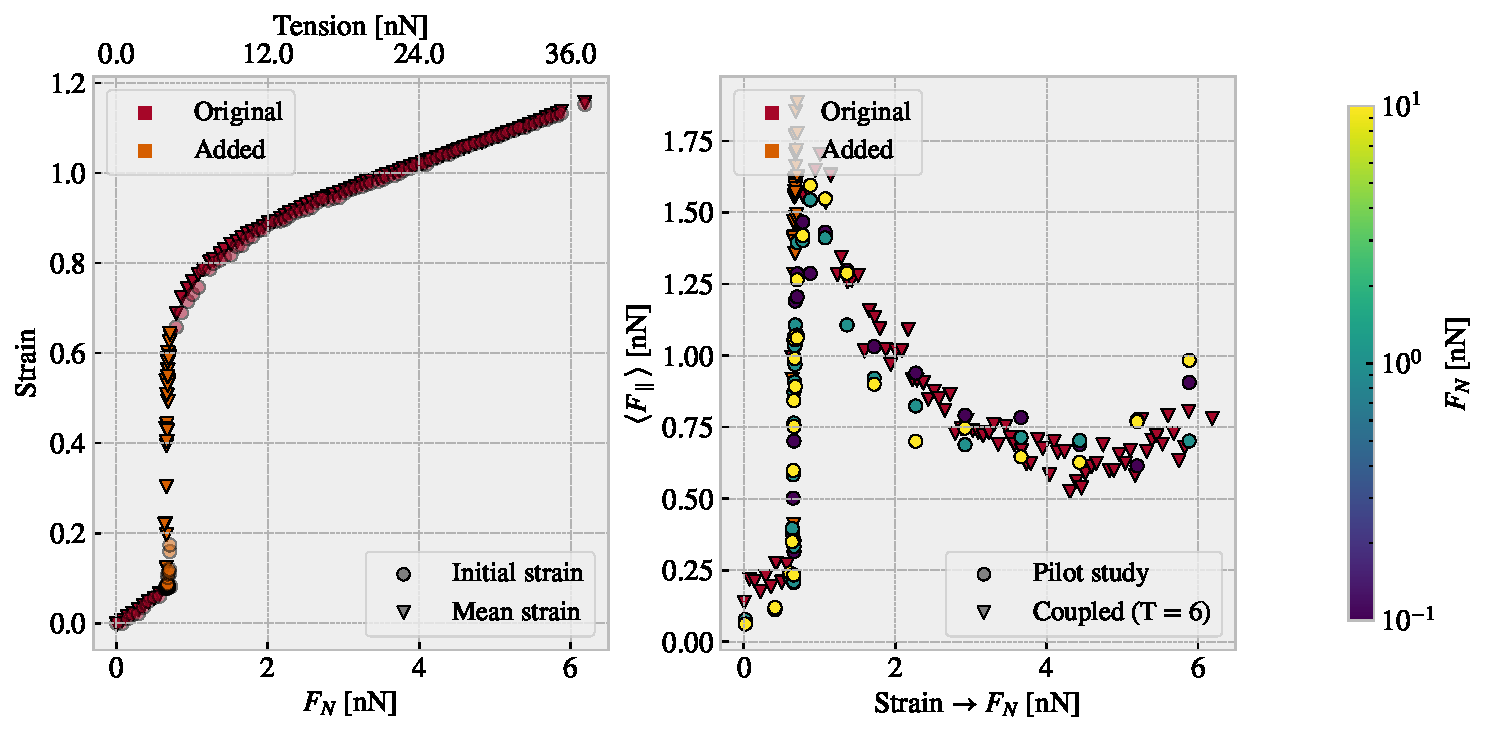
\includegraphics[width=\linewidth]{../thesis/figures/negative_coefficient/manual_coupling_tension_hon2215.pdf}	
	\caption{Honeycomb $(2,2,1,5)$}
	\end{figure}	
\end{frame}
%
%%% New frame %%%
%
\begin{frame}{Negative friction coefficient}
	\framesubtitle{Honeycomb deformations}
	% \begin{figure}
	% 	\centering    
	% 	\movie[open,showcontrols=true]{\includegraphics[width=\textwidth, keepaspectratio]{figures/hon_stretch.png}}{figures/hon_stretch.mov}
	% 	\caption{Honeycomb $(2,2,1,5)$ stretch.}
	% \end{figure} 
	\begin{figure}
		\centering    
		\movie[open,showcontrols=true]{\includegraphics[width=0.70\textwidth, keepaspectratio]{figures/hon_stretch2.png}}{figures/hon_stretch_anim/anim.mov}
		% \caption{Honeycomb $(2,2,1,5)$ stretch.}
	\end{figure} 
\end{frame}

%
%%% New frame %%%
%
\section{Kirigami pattern search} %%%%%%%%%%%%%%%%%%%%%%%%%%%%%%%%%%%%%%%%%%%%%%%%%%%%%%%%%%%%%
\begin{frame}{Kirigami pattern search}
    \tableofcontents[currentsection]
\end{frame}
%
%%% New frame %%%
%
% \subsection{Machine learning}
\begin{frame}{Machine learning}
	Dataset
	\begin{itemize}
		\item 216 Kirigami configurations ($\sim 10,000$ data points)
	\end{itemize}
	\vspace*{5mm}
	Machine learning
	\begin{itemize}
		\item Input: Kirigami configuration, strain and load
		\item Output: Mean friction, rupture
		% \item Output: \underline{Mean $F_{\text{fric}}$}, $\max \ F_{\text{fric}}$, contact area, porosity, \underline{rupture}, rupture strain
	\end{itemize}

	\begin{figure}[H]
		\centering
		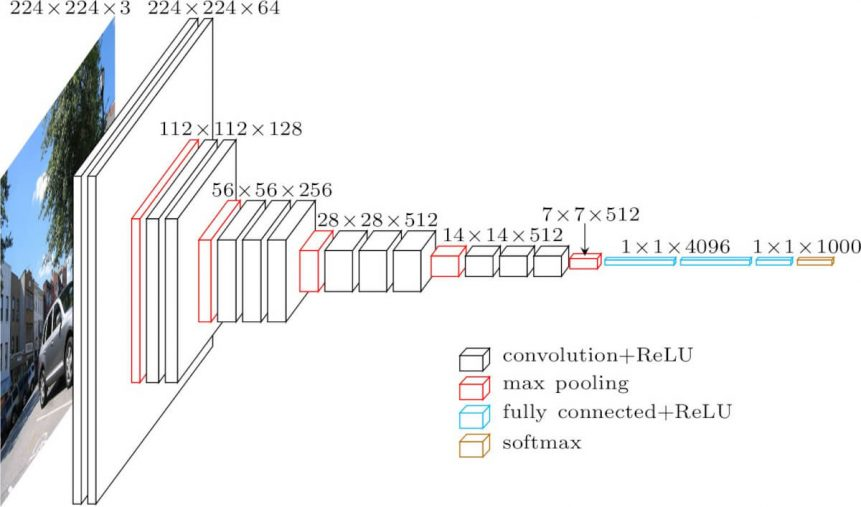
\includegraphics[width=0.5\linewidth]{../thesis/figures/ML/VGGNet16.jpg}
		\caption{Convolutional neural network. Reproduced from~\cite{VGGNet_16_image}.}
	\end{figure}
\end{frame}
%
%%% New frame %%%
%
% \begin{frame}{Dataset}
% 	\framesubtitle{Correlation}
% 	\begin{figure}[H]
% 		\centering
% 		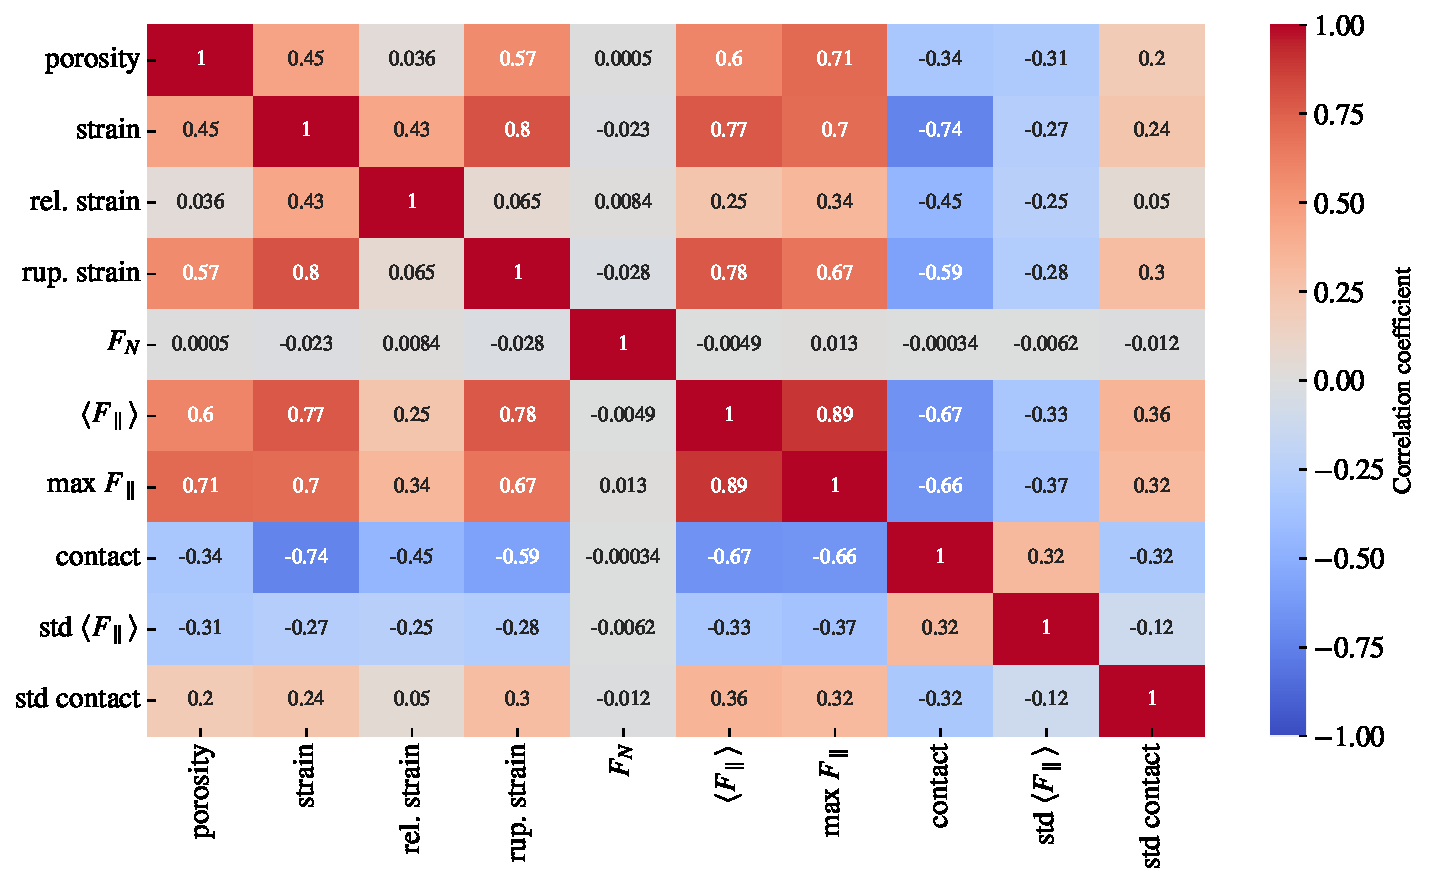
\includegraphics[width=0.9\linewidth]{../thesis/figures/ML/corrcoef_matrix.pdf}
% 		\caption{Pearson product-moment correlation coefficients. }
% 	  \end{figure}
% \end{frame}
%
%%% New frame %%%
%
% \begin{frame}{Machine learning}
% 	\framesubtitle{Results}
% 	\begin{itemize}
% 		\item Validation $R^2$ score $\sim 98 \%$
% 	\end{itemize}

% 	\begin{figure}[H]
% 		\centering
% 		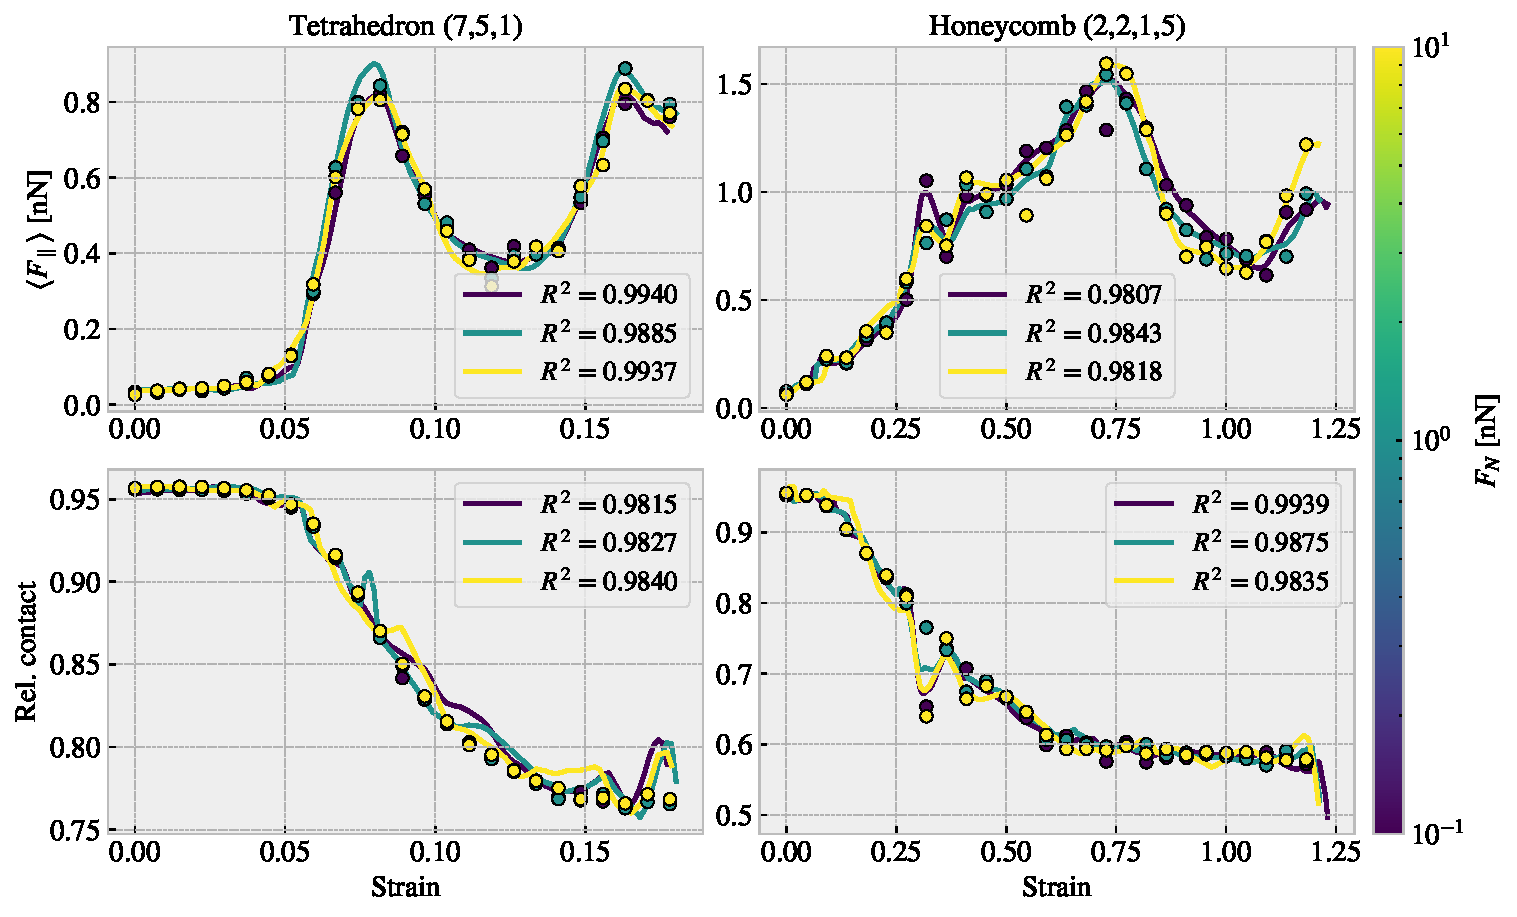
\includegraphics[width=0.8\linewidth]{../figures/final_model_evaluation_slide.pdf}
% 		\caption{Visual evaluation of the final model predictions on the Tetrahedron $(7,5,1)$ and Honeycomb $(2,2,1,5)$ used in the pilot study.}
% 	\end{figure}  
% \end{frame}

%
%%% New frame %%%
%
% \subsection{Accelerated search for new designs}
\begin{frame}{Properties of interest}
	\begin{align*}
		&\text{(1) } \min F_{\text{fric}},& &\text{(2) } \max F_{\text{fric}},& &\text{(3) } \max \Delta F_{\text{fric}},& &\text{(4) } \max \text{drop}.&
	\end{align*}
	\begin{figure}[H]
		\centering
		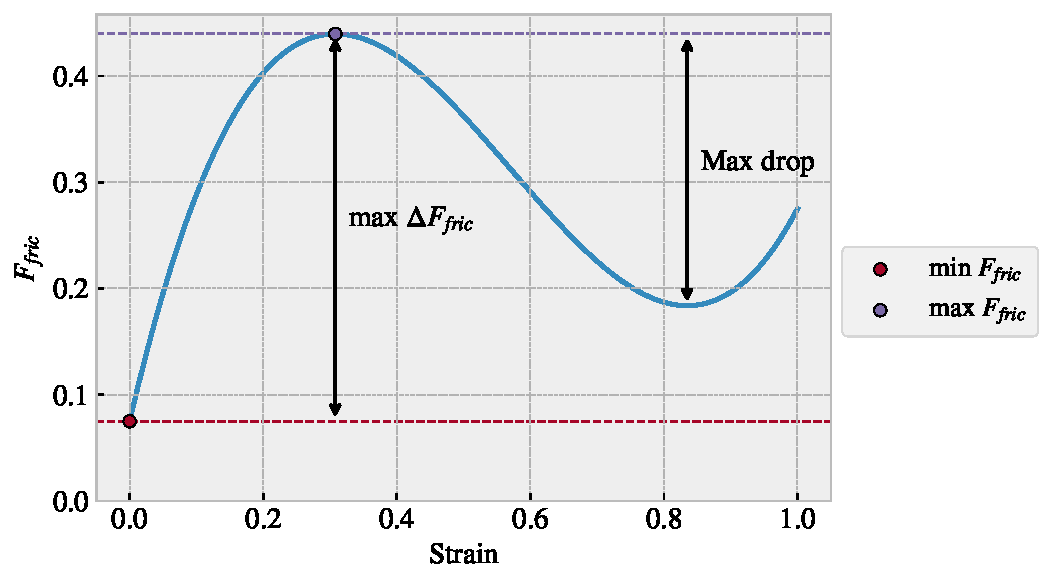
\includegraphics[width=0.8\linewidth]{figures/prop_of_interets.pdf}
		\caption{Properties of interest.}
	\end{figure}
\end{frame}
%
%%% New frame %%%
%
\begin{frame}{Accelerated search for new designs}
	% \framesubtitle{Extended dataset}
	Two search approaches
	\begin{enumerate}
		\item Extended dataset search
		\begin{align*}
			&\text{Tetrahedron:} \ \num{1.35e5},& &\text{Honeycomb:} \ \num{2.025e6},& &\text{Random walk:} \ \num{e4}&
		\end{align*}
		% \begin{itemize}
		% 	\item Tetrahedron: \num{1.35e5} configurations 
		% 	\item Honeycomb: \num{2.025e6} configurations
		% 	\item Random walk: \num{e4} configurations
		% \end{itemize}
		\item Genetic algorithm
		\begin{itemize}
			\item Survival of the fittest 
			% \item Max drop property optimization 
		\end{itemize}
	\end{enumerate}

	% \begin{figure}[H]
	% 	\centering
	% 	\includegraphics[width=0.5\linewidth]{../thesis/figures/search/RW_search_top5.png}
	% 	\caption{Top 5 candidates for random walk extended dataset accelerated search. }
	% \end{figure}  
\end{frame}
%
%%% New frame %%%
%






% \begin{frame}{Dataset}
% 	% \footnotesize
% 	\begin{table}[H]
% 		\begin{center}
% 		\caption{Summary of the generated data points in the dataset.}
% 		\begin{tabular}{ | c | c | c | c |} \hline
% 		\textbf{Type} & \textbf{Configurations} & \textbf{Data points} & \textbf{Ruptures} \\ \hline
% 		Pilot study & 3 & 261 & \: 25 \: (9.58 \%)\\ \hline
% 		Tetrahedron & 68 &  3015 & 391 (12.97 \%)\\ \hline
% 		Honeycomb & 45 &  1983 & \: 80 \: (4.03 \%)\\ \hline
% 		Random walk & 100 &  4401 & 622 (14.13 \%) \\ \Xhline{2\arrayrulewidth}
% 		Total & 214 (216) &  9660 & 1118 (11.57 \%) \\ \hline
% 		\end{tabular}
% 		\end{center}
% 	\end{table}
% \end{frame}

% \begin{frame}{Dataset}
% 	\framesubtitle{Properties of interest}
% 	Properties of interest
% 	\begin{align*}
% 		&\text{(1) } \min F_{\text{fric}},& &\text{(2) } \max F_{\text{fric}},& &\text{(3) } \max \Delta F_{\text{fric}},& &\text{(4) } \max \text{drop}.&
% 	\end{align*}
% 	\begin{figure}[H]
% 		\centering
% 		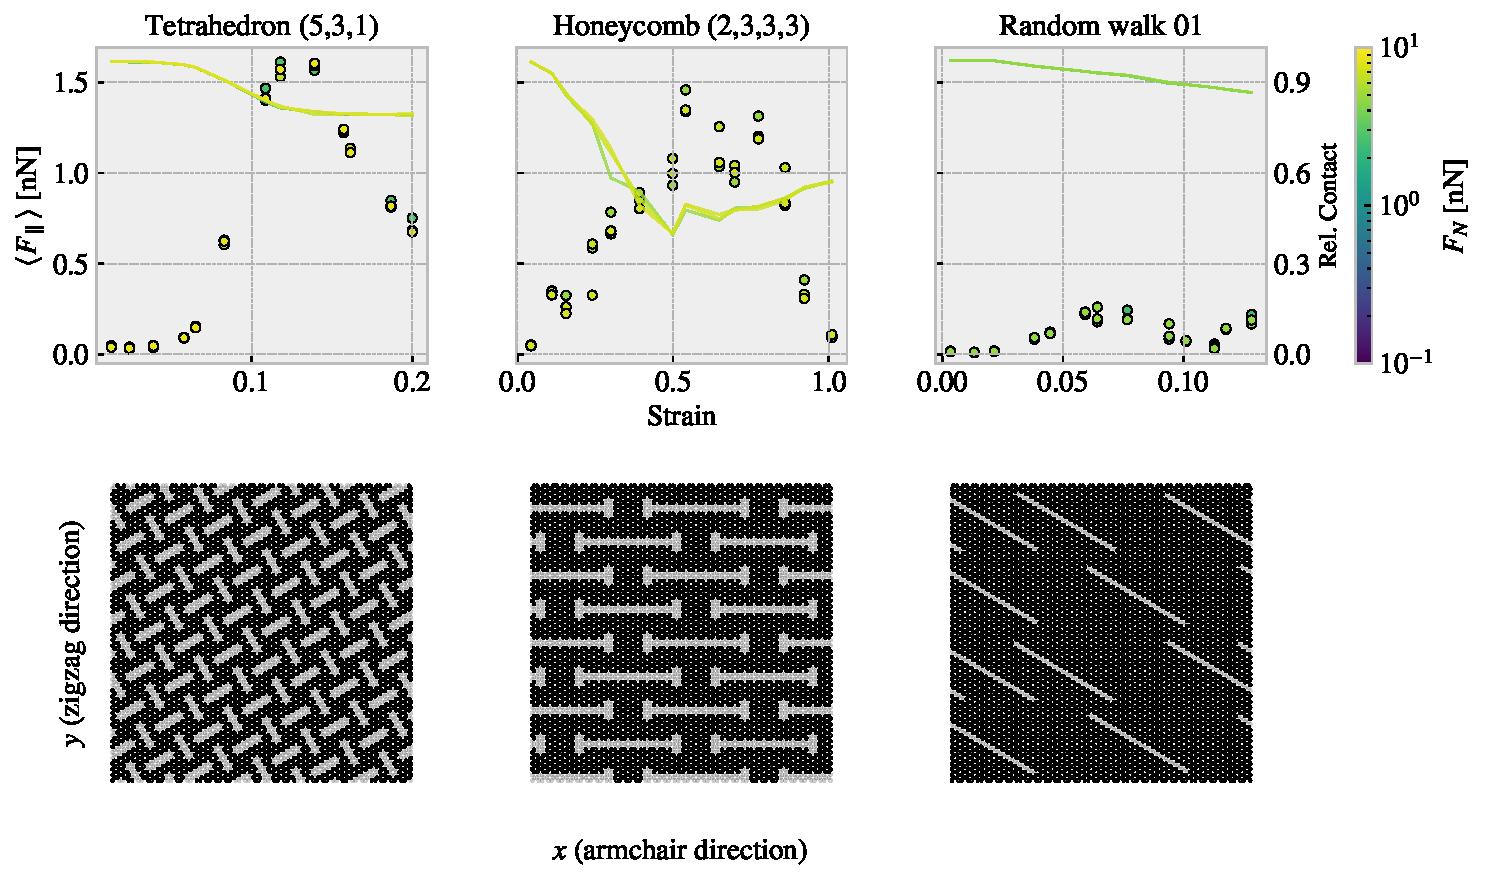
\includegraphics[width=0.7\linewidth]{../thesis/figures/stretch_profiles/PP_max_drop.pdf}
% 		\caption{Max drop property. Best candidates in the dataset.}
% 	  \end{figure}
% \end{frame}
%
%%% New frame %%%
%
% \begin{frame}{Machine learning}
% 	\begin{itemize}
% 		\item Convolutional neural network
% 		\item Input: Kirigami configuration, strain and load
% 		\item Output: \underline{Mean friction}, maximum friction, contact area, porosity, \underline{rupture}, rupture strain
% 	\end{itemize}

% 	\begin{figure}[H]
% 		\centering
% 		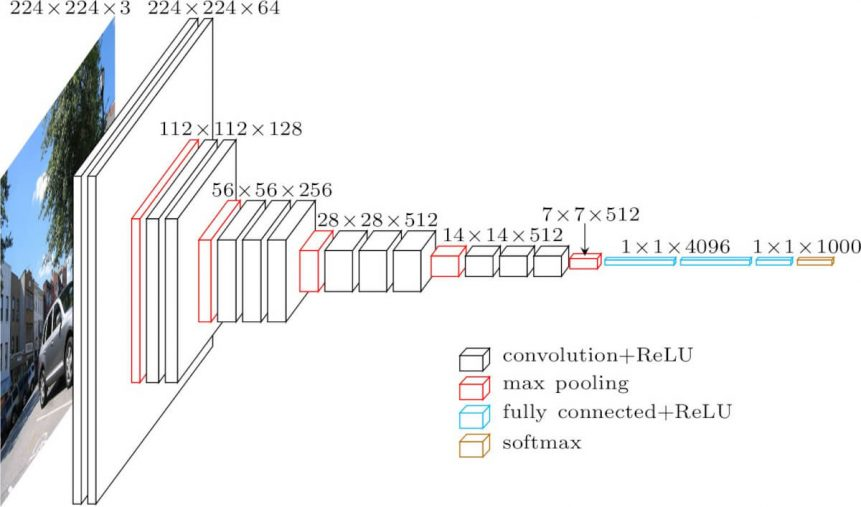
\includegraphics[width=0.5\linewidth]{../thesis/figures/ML/VGGNet16.jpg}
% 		\caption{VGGNet-16 network convolutional network architecture. Reproduced from~\cite{VGGNet_16_image}.}
% 	  \end{figure}
% \end{frame}
%
%%% New frame %%%
%
% \begin{frame}{Machine learning}
% 	\framesubtitle{Model performance}

% 	\begin{table}[H]
% 		\begin{center}
% 		\footnotesize
% 		\caption{Evaluation of the final model performance.}
% 		\label{tab:final_model_eval}
% 		\begin{tabular}{ | c | c | c | c | c | c | c |} \hline
% 		  & \multicolumn{3}{c|}{$R^2$ [\num{e2}]} & Abs. [\num{e2}] & Rel. [\num{e2}]  & Acc. [\num{e2}] \\ \hline
% 		  & Mean $F_f$ & Max $F_f$ & Contact & Porosity & Rup.\ Strain & Rupture \\ \hline
% 		Validation  & 98.067 & 93.558 & 94.598 & 2.325 & 12.958 & 96.102 \\ \hline
% 		Tetrahedron & 88.662 & 85.836 & 64.683 & 1.207 & \phantom{0}5.880 & 99.762 \\ \hline
% 		Honeycomb   & 96.627 & 89.696 & 97.171 & 1.040 & \phantom{0}1.483 & 99.111 \\ \hline
% 		\end{tabular}
% 		\end{center}
% 	\end{table}
% \end{frame}
% %
%%% New frame %%%
%
% \begin{frame}{Machine learning}
% 	\framesubtitle{Model performance}
% 	\begin{figure}[H]
% 		\centering
% 		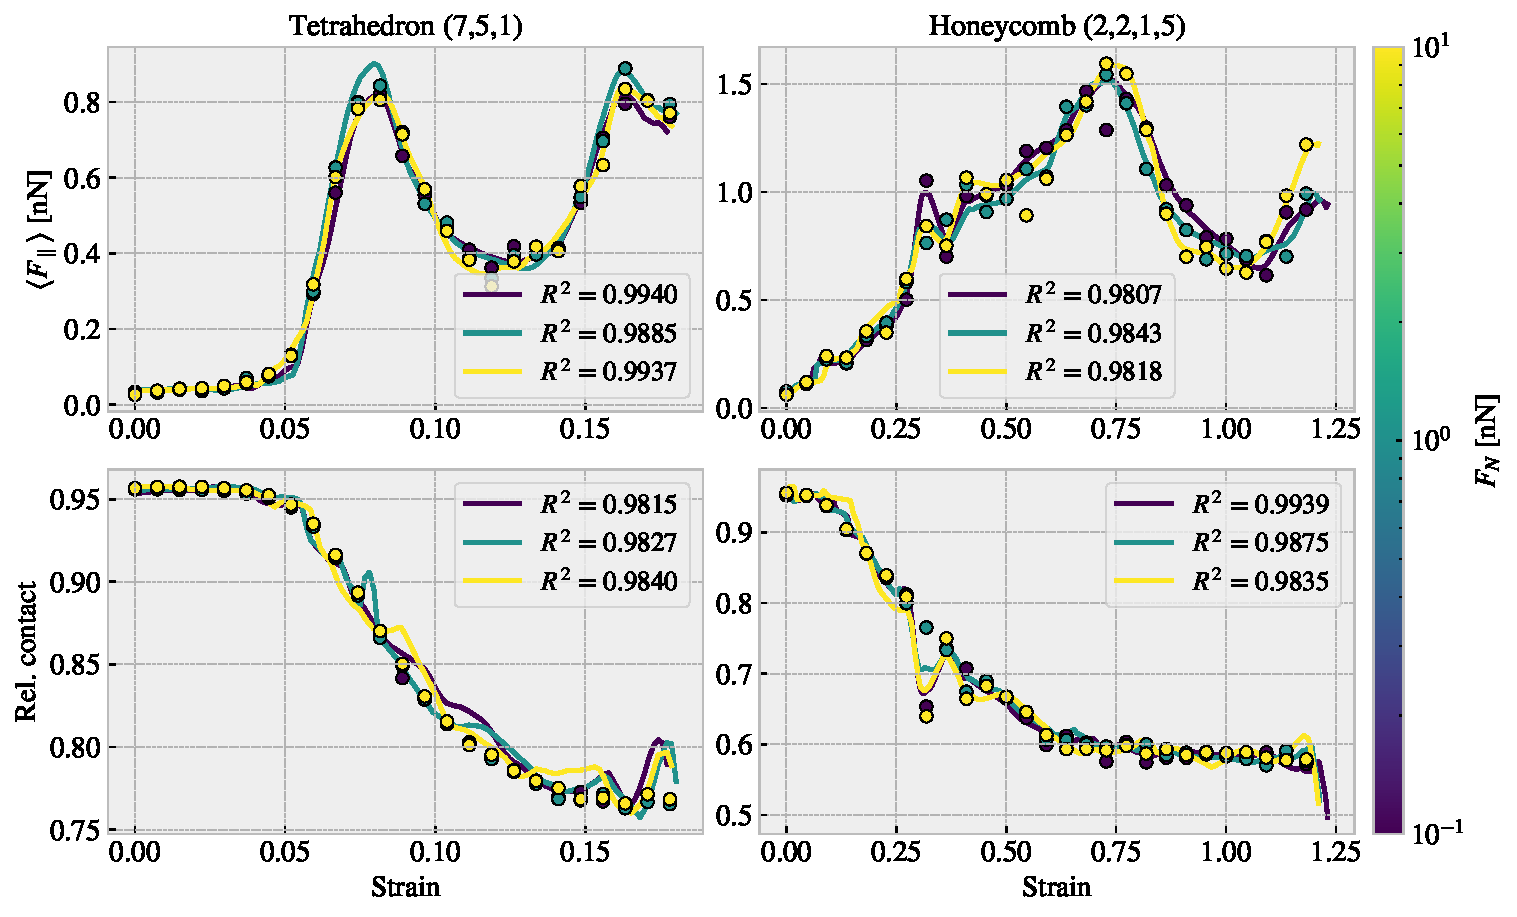
\includegraphics[width=0.8\linewidth]{../figures/final_model_evaluation_slide.pdf}
% 		\caption{Visual evaluation of the final model predictions on the Tetrahedron $(7,5,1)$ and Honeycomb $(2,2,1,5)$ used in the pilot study.}
% 	\end{figure}  

% \end{frame}
%
%%% New frame %%%
%
% \begin{frame}{Accelerated search}
% 	\framesubtitle{Extended dataset}
% 	\begin{itemize}
% 		\item Tetrahedron: \num{1.35e5} configurations 
% 		\item Honeycomb: \num{2.025e6} configurations
% 		\item Random walk: \num{e4} configurations
% 	\end{itemize}


% 	\begin{table}[H]
% 		\begin{center}
% 		% \caption{Results for the accelerated search using the pattern generators. The top search candidates for each of the four properties of interest are shown in the left section (Search) regarding the Tetrahedron, Honeycomb and Random walk patterns respectively. The upper rows show the scores and the lower rows the associated names (parameters). The right section (Data) shows the corresponding scores from the best candidates within the dataset (from~\cref{tab:data_properties}). All scores are given in units nN.}
% 		\begin{tabular}{|L{1.75cm} |c|c|c| } \cline{2-4}
% 		\multicolumn{1}{c|}{\textbf{Search Pred.}} & Tetrahedron & Honeycomb & Random walk \\ \hline
% 		$\min F_{\text{fric}}$         & $-0.062 \ \ $  & $-0.109 \ \ $  & $-0.061 \ \ $ \\ \hline
% 		$\max F_{\text{fric}}$         & $1.089$        & $2.917$        & $0.660$       \\ \hline
% 		$\max \Delta F_{\text{fric}}$  & $1.062$        & $2.081$        & $0.629$       \\ \hline
% 		max drop                       & $0.277$        & $1.250$        & $0.269$       \\ \hline
% 		\multicolumn{4}{c|}{} \\ \cline{2-4}
% 		\multicolumn{1}{c|}{\textbf{Original}} & Tetrahedron & Honeycomb & Random walk \\ \hline
% 		$\min F_{\text{fric}}$         	& 0.0067 & 0.0177 & 0.0024 \\ \hline 
% 		$\max F_{\text{fric}}$         	& 1.5875 & 2.8903 & 0.5758 \\ \hline 
% 		$\max \Delta F_{\text{fric}}$ 	& 1.5529 & 2.0234 & 0.5448 \\ \hline 
% 		max drop    					& 0.8841 & 1.2785 & 0.1818 \\ \hline 
% 		\end{tabular}
% 		\end{center}
% 	\end{table}

% \end{frame}
% \begin{frame}{Accelerated search}
% 	% \framesubtitle{Extended dataset}
% 	\begin{enumerate}
% 		\item Extended dataset search
% 		\begin{itemize}
% 			\item Tetrahedron: \num{1.35e5} configurations 
% 			\item Honeycomb: \num{2.025e6} configurations
% 			\item Random walk: \num{e4} configurations
% 		\end{itemize}
% 		\item Genetic algorithm
% 		\begin{itemize}
% 			\item Max drop property optimization 
% 		\end{itemize}
% 	\end{enumerate}

% 	\begin{figure}[H]
% 		\centering
% 		\includegraphics[width=0.5\linewidth]{../thesis/figures/search/RW_search_top5.png}
% 		\caption{Top 5 candidates for random walk extended dataset accelerated search. }
% 	\end{figure}  
% \end{frame}
%
%%% New frame %%%
%
% \begin{frame}{Accelerated search}
% 	\framesubtitle{Grad-CAM}
% 	\begin{figure}[H]
% 		\centering
% 		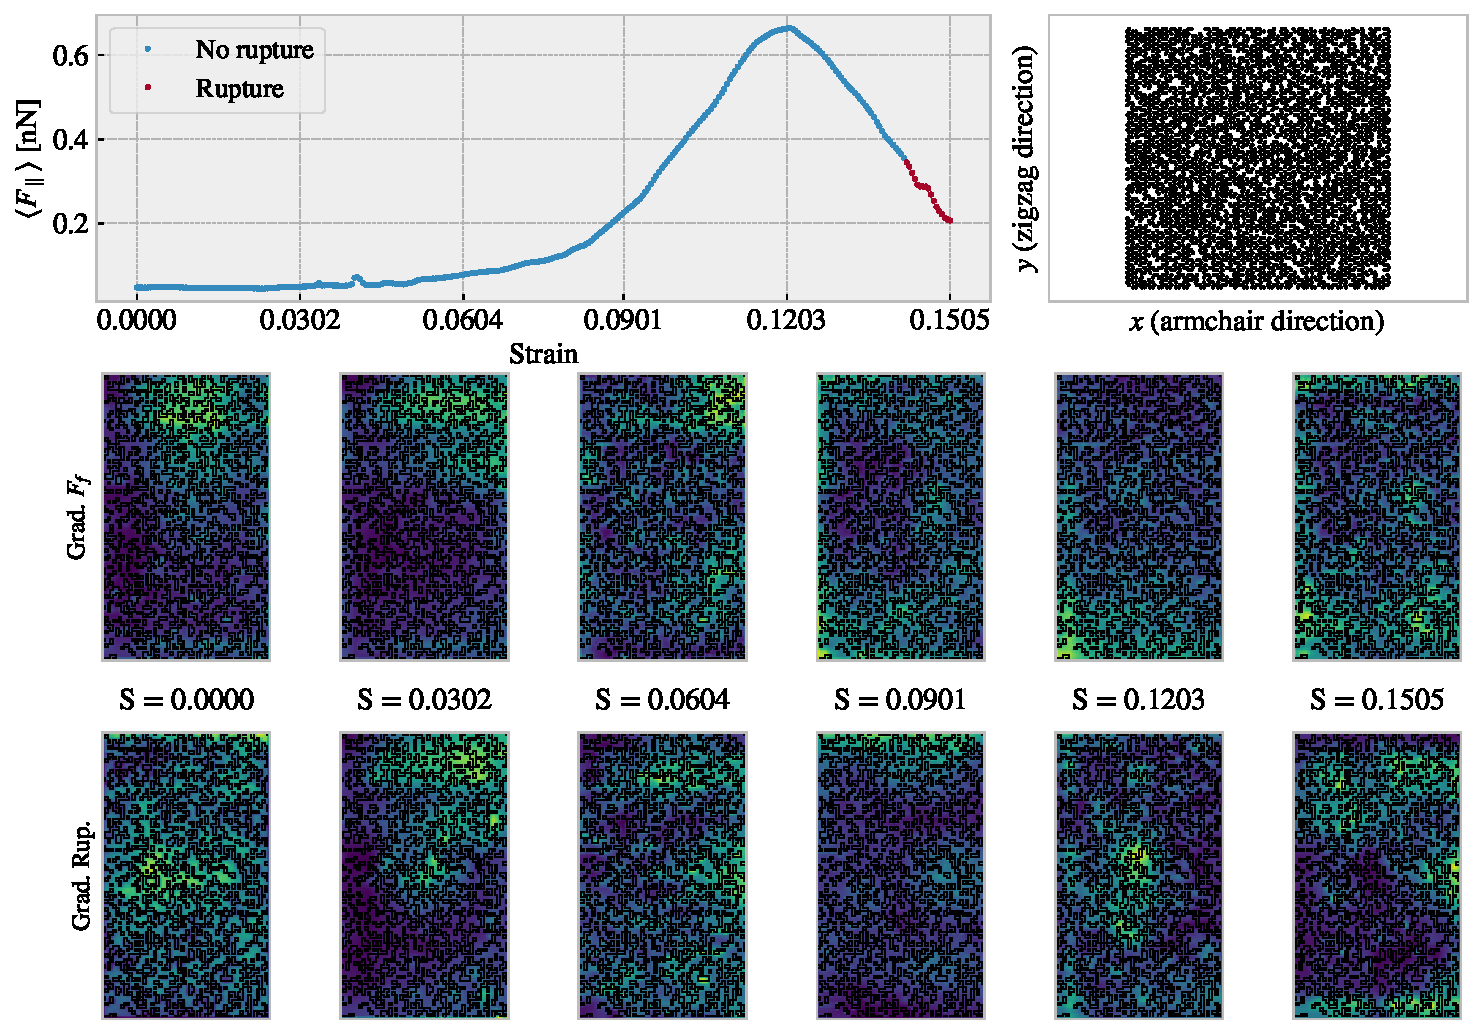
\includegraphics[width=0.7\linewidth]{../thesis/figures/search/grad_cam_GA_RN_start_top0.pdf}
% 		\caption{Genetic algorithm suggestion from a mixed porosity start. Top: Friction-strain curve and configuration. Bottom: Grad-CAM analysis.}
% 	\end{figure}  
% \end{frame}
%
%%% New frame %%%
%
\begin{frame}{Accelerated search}
	\framesubtitle{Grad-CAM}
	\begin{figure}[H]
		\centering
		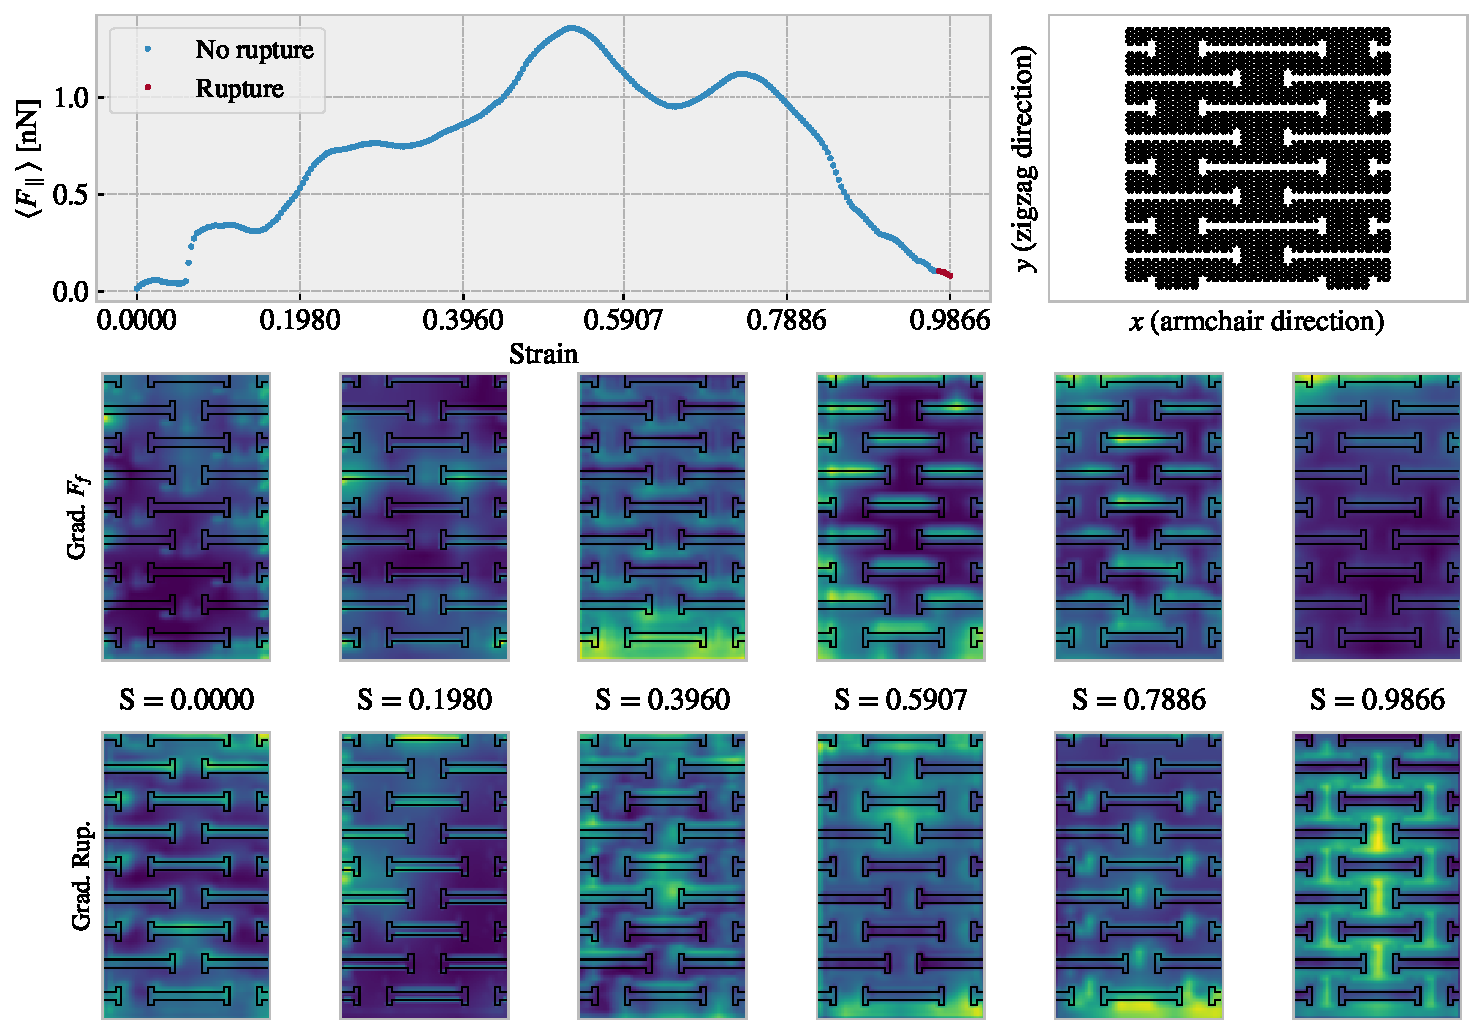
\includegraphics[width=0.7\linewidth]{../thesis/figures/search/grad_cam_hon_3_3_5_3_12_0.pdf}
		\caption{Honeycomb $(3,3,5,3)$. Top: Friction-strain curve and configuration. Bottom: Grad-CAM analysis.}
	\end{figure}  
\end{frame}
%
%%% New frame %%%
%



\section{Summary and outlook} %%%%%%%%%%%%%%%%%%%%%%%%%%%%%%%%%%%%%%%%%%%%%%%%%%%%%%%%%%%%%
\begin{frame}{Outline}
    \tableofcontents[currentsection]
\end{frame}


\begin{frame}{Summary and outlook}


	\begin{columns} 
		% \hspace{5mm}
		\begin{column}{.5\textwidth}
			Key findings		
			\begin{itemize}
				\item Non-monotonous friction-strain
				\item Negative friction coefficient
				\item Machine learning needs more data
			\end{itemize}
			\vspace*{5mm}
			Further studies
			\begin{itemize}
				\item Underlying mechanism
				\begin{itemize}
					\item Commensurability hypothesis
				\end{itemize}
				\item Friction-strain relationship at different physical conditions
				\item Edge and thermostat effects
				\item Improve dataset with active learning 
			\end{itemize}
		\end{column}
		\begin{column}{.5\textwidth}

			\begin{figure}[H]
				\centering
				\begin{subfigure}[b]{\textwidth}
					\centering
					\includegraphics[width=\textwidth]{figures/friction_strain_summary.pdf}
				\end{subfigure}
				\begin{subfigure}[b]{\textwidth}
					\centering
					\includegraphics[trim={10.5cm 0 0 0.5cm},clip,width=0.8\linewidth]{../thesis/figures/negative_coefficient/manual_coupling_tension_hon2215.pdf}	
				\end{subfigure}
				% \caption{Qualitative illustration of microscopic asperity deformation under increasing load. Reproduced from~\cite{wiki:asperities}.}
			\end{figure}
		\end{column}%
	\end{columns}




\end{frame}


\FinalFrame



\begin{frame}%[allowframebreaks]
	\frametitle{References}
	\printbibliography
	% \bibliographystyle{apalike}
	% \bibliographystyle{plain}
	% \printbibliography
	% \bibliography{./presentation/bibliography.bib}
\end{frame}



\end{document} 


